% Adapted from the author's public Erdos Paper IV v1.23 series_template.tex.
% Layout provenance is recorded in 02_validation; the Markdown is semantic authority.
\documentclass[spanish,11pt,a4paper]{article}
\usepackage[margin=1in]{geometry}
\usepackage{fontspec}
\setmainfont{lmroman10-regular.otf}[BoldFont=lmroman10-bold.otf,ItalicFont=lmroman10-italic.otf,BoldItalicFont=lmroman10-bolditalic.otf]
\setsansfont{lmsans10-regular.otf}[BoldFont=lmsans10-bold.otf]
\setmonofont{lmmono10-regular.otf}[Scale=MatchLowercase]
\usepackage{amsmath,amssymb}
\providecommand{\mathscr}{\mathcal}
\usepackage[spanish,es-noshorthands,es-tabla]{babel}
\usepackage{microtype,parskip}
\usepackage{longtable,booktabs,array,calc}
\usepackage{xcolor,xurl}
\usepackage{hyperref,bookmark}
\usepackage{etoolbox,needspace}
\setcounter{secnumdepth}{-\maxdimen}
\setlength{\emergencystretch}{3em}
\providecommand{\tightlist}{\setlength{\itemsep}{0pt}\setlength{\parskip}{0pt}}
\newcounter{none}
\AtBeginEnvironment{longtable}{\Needspace{8\baselineskip}\small}
\pretocmd{\section}{\Needspace{5\baselineskip}}{}{}
\pretocmd{\subsection}{\Needspace{4\baselineskip}}{}{}
\pretocmd{\subsubsection}{\Needspace{4\baselineskip}}{}{}
\urlstyle{same}
\usepackage{graphicx,float}
\hypersetup{pdftitle={Descomposiciones en triángulos III: Absorción tipada física y estadísticas prescritas},pdfauthor={Juan Pablo Traverso Gianini},pdflang={es-ES},colorlinks=true,linkcolor=blue,urlcolor=blue,citecolor=blue}
\title{Descomposiciones en triángulos III: Absorción tipada física y estadísticas prescritas}
\author{Juan Pablo Traverso Gianini\\
\small Investigador independiente, Santiago, Chile\\
\small \href{mailto:jtraverso@gmail.com}{jtraverso@gmail.com}\\
\small ORCID: 0009-0003-6068-4096}
\date{}\begin{document}\raggedbottom\maketitle
\textbf{Paper III de la serie Descomposiciones en triángulos.}\\
\textbf{Preprint 1.0 --- 1 de noviembre de 2026.}

\subsection{Resumen}\label{resumen}

Estudiamos particiones de las aristas de un grafo en triángulos con combinaciones prescritas de etiquetas en sus vértices. Establecemos, con pruebas completas verificadas en Lean, un criterio suficiente basado en cuatro condiciones: una cobertura fraccionaria exacta y positiva, pertenencia al retículo entero de los triángulos existentes, muchos vecinos comunes tipados y suficientes intercambios locales llamados bisagras. La construcción prepara reservas descomponibles antes de conocer las aristas que quedarán sin cubrir. Cada reserva, certificado e intercambio está dentro del grafo. El criterio es una variante del marco particionado anunciado por Delcourt y Postle, con hipótesis fraccionarias y de retículo más fuertes y una normalización explícita del conteo de bisagras con raíces fijadas.

Un teorema reforzado controla las estadísticas lineales de triángulos y las configuraciones de Pasch en una misma descomposición; los objetivos vienen dados por la cobertura fraccionaria original. Las aplicaciones proporcionan cuadrados latinos cuyos perfiles determinan los objetivos de intercalados, y refinamientos estadísticos de descomposiciones conocidas del grafo pentapartito completo \(K_{s,s,s,s,s}\) para \(3\mid s\). Para las estadísticas lineales de triángulos por separado, la Sección 7 da una cota de torre computable que depende de los parámetros de T+.

Las pruebas generales completas están en la formalización Lean adjunta, cuya instantánea de fuentes superó la reconstrucción y las auditorías de axiomas de los resultados finales. El artículo explica la construcción y demuestra las aplicaciones.

\textbf{Palabras clave:} descomposición en triángulos; grafos etiquetados; absorción; retículo entero; cuadrado latino; configuración de Pasch.

\subsection{1. Introducción}\label{introducciuxf3n}

Asignemos una etiqueta a cada vértice de un grafo y fijemos los multiconjuntos de tres etiquetas permitidos. Queremos dividir las aristas en triángulos con esas etiquetas. Un multiconjunto permitido puede repetir una etiqueta, pero cada triángulo tiene tres vértices distintos. Las etiquetas corresponden a los vértices, no a las aristas.

Nuestro resultado principal da cuatro condiciones suficientes. Se refieren al grafo concreto y a sus triángulos permitidos. La sección 2 presenta sus definiciones precisas.

{\Needspace{18\baselineskip}\begin{longtable}[]{@{}
  >{\raggedright\arraybackslash}p{(\linewidth - 4\tabcolsep) * \real{0.3333}}
  >{\raggedright\arraybackslash}p{(\linewidth - 4\tabcolsep) * \real{0.3333}}
  >{\raggedright\arraybackslash}p{(\linewidth - 4\tabcolsep) * \real{0.3333}}@{}}
\toprule\noalign{}
\begin{minipage}[b]{\linewidth}\raggedright
Condición
\end{minipage} & \begin{minipage}[b]{\linewidth}\raggedright
Qué proporciona
\end{minipage} & \begin{minipage}[b]{\linewidth}\raggedright
Uso en la construcción
\end{minipage} \\
\midrule\noalign{}
\endhead
\bottomrule\noalign{}
\endlastfoot
H1: una semilla fraccionaria exacta y difusa & Pesos positivos de triángulos, del orden de \(1/n\), que suman uno en cada arista & Un punto de partida exacto para el empaquetamiento aproximado y las correcciones posteriores \\
H2: el retículo entero de triángulos físicos & Una combinación entera de triángulos existentes igual al vector de aristas & La compatibilidad entera necesaria para la absorción \\
H3: vecinos comunes tipados & Muchas elecciones de un vértice con la etiqueta requerida & La colocación de las piezas locales \\
H4: bisagras físicas & Muchos grafos auxiliares acotados que admiten dos descomposiciones locales alternativas & El cambio de triángulos sin perder la posibilidad de descomponer \\
\end{longtable}
}

Estas cuatro condiciones se verifican en el grafo concreto; no se supone ninguna descomposición previa ni ningún absorbedor externo. Aquí \(n\) es el número de vértices, \(I\) el conjunto de etiquetas y \(\mathcal F\) la familia permitida. Las constantes \(C\), \(\alpha\) y \(h\) controlan, respectivamente, las cotas de la semilla, la disponibilidad local y el orden máximo de las bisagras.

\Needspace{7\baselineskip}\textbf{Teorema T.} Fijemos \(I,\mathcal F,\alpha,C,h\) con \(\alpha>0\), \(C\geq1\) y \(h\geq6\). Existe un entero \(n_0\) tal que todo grafo etiquetado G de orden \(n\geq n_0\) que satisface H1--H4 admite una descomposición en triángulos permitidos.

El teorema reforzado T+, en la sección 2.3, produce una descomposición que además respeta estadísticas prescritas de triángulos y un número prescrito de configuraciones de Pasch, formadas por cuatro triángulos. Ambos objetivos proceden de la semilla fraccionaria original. Una misma descomposición satisface todas las estimaciones solicitadas.

\subsubsection{1.1. Absorción dentro del grafo}\label{absorciuxf3n-dentro-del-grafo}

La absorción prepara la respuesta a las aristas que deja una descomposición aproximada. Se reserva un pequeño grafo R antes de conocer el residuo M. La reserva tiene una descomposición propia; también puede descomponerse junto con cualquier residuo que cumpla condiciones especificadas de soporte, retículo y tamaño. Llamamos admisible a un residuo de este tipo; la Sección 5.1 precisa la clase terminal. Tras cubrir el resto del grafo, se utiliza esta segunda descomposición para terminar. La dificultad es preparar una reserva que sirva para todos los residuos que pueda producir la construcción.

En una construcción iterativa, las rondas sucesivas trasladan las aristas sin cubrir a conjuntos de vértices más pequeños. La absorción refinada, desarrollada por Delcourt y Postle {[}6{]} y expuesta posteriormente por Postle {[}7{]}, organiza muchas elecciones locales de absorción con solapamiento controlado. La iteración controla dónde queda el residuo; el refinamiento controla los recursos locales necesarios para absorberlo.

Nuestro trabajo sigue esta dirección. El adjetivo \emph{física} precisa cómo se realizan los objetos: cada certificado usa triángulos presentes en el grafo, cada arista auxiliar pertenece a él y cada sustitución local respeta las etiquetas permitidas. Una identidad entre conteos de etiquetas no basta. Incluso una identidad entera entre triángulos existentes puede tener coeficientes negativos; la construcción debe realizarla mediante descomposiciones efectivas. La sección 3 explica este paso.

Los Papers I y II {[}1, 2{]} proporcionan las construcciones en que se apoya el argumento. Paper II desarrolla las correcciones tipadas y las piezas de absorción; Paper I organiza las rondas de cobertura protegida y su iteración. Aquí conservamos esas estructuras en el grafo que efectivamente queda después de cada ronda y añadimos el control estadístico hasta completar la descomposición. Las reservas y las colecciones de piezas de corrección se obtienen en la demostración; no son supuestos adicionales de T.

La figura \ref{fig:architecture} distingue la reserva elegida una sola vez de los recursos de corrección utilizados durante las rondas.

\begin{figure}[H]
\centering
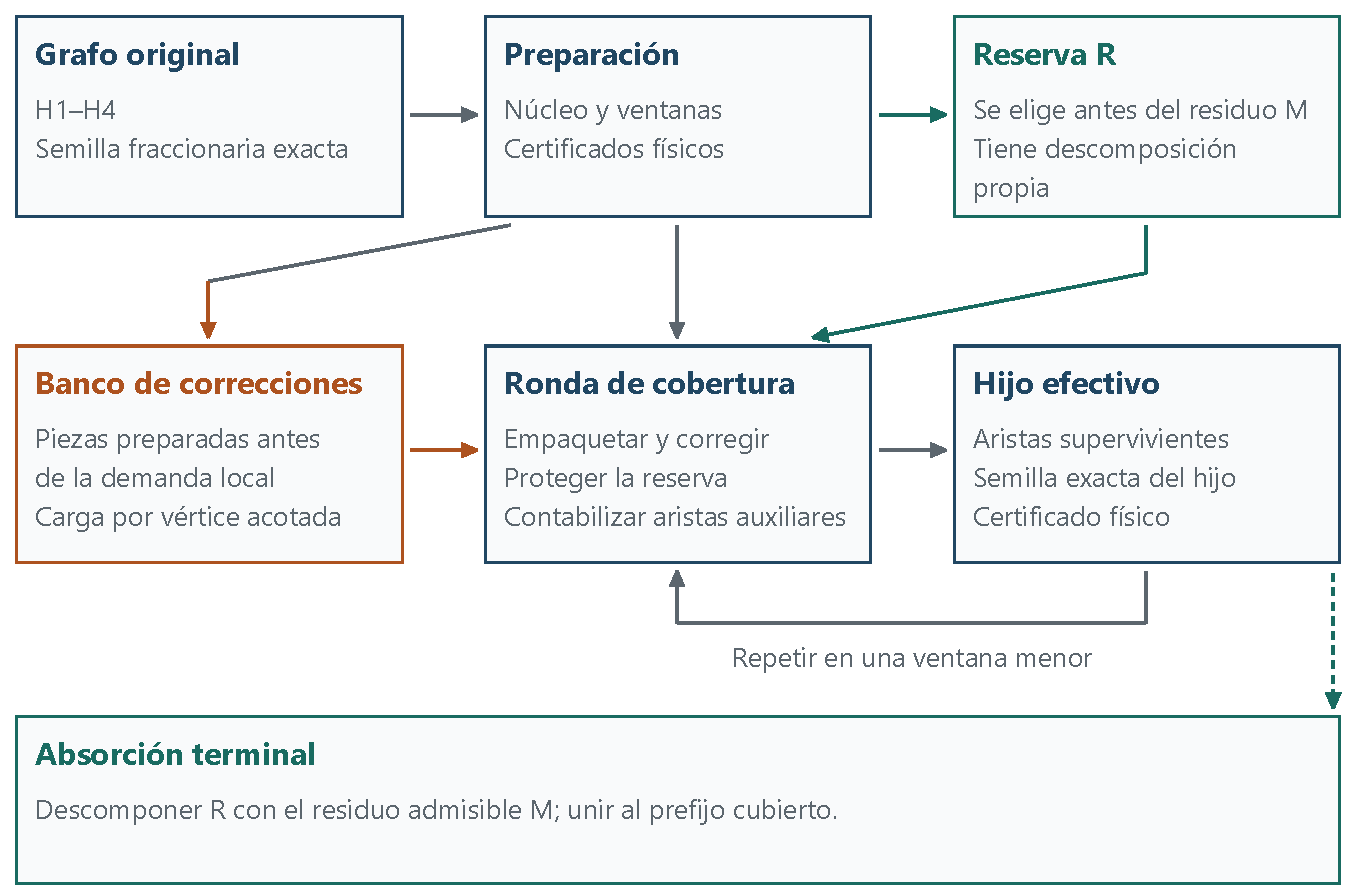
\includegraphics[width=0.98\linewidth]{figures/architecture_es.pdf}
\caption{Orden esquemático de la construcción. La preparación proporciona la reserva y los recursos de corrección antes de conocer las demandas correspondientes. Cada ronda deja un hijo efectivo con semilla exacta; la iteración conserva la reserva terminal hasta absorber el residuo. Las flechas indican dependencias, no inclusiones ni tamaños relativos.}
\label{fig:architecture}
\end{figure}

\subsubsection{1.2. Aplicaciones y trabajos relacionados}\label{aplicaciones-y-trabajos-relacionados}

El teorema de Keevash para complejos etiquetados {[}15, Teorema 3.1; 3, Teorema 4.18{]} exige regularidad, pertenencia al retículo y extensibilidad con raíces fijadas. Aplicarlo a T requeriría una traducción que verificase esas condiciones. No afirmamos esa reducción ni una mayor generalidad. El criterio enunciado más próximo es Delcourt--Postle {[}14, Teorema 13.16{]}. Para triángulos particionados, H3 es su condición anti-edgeful, y nuestra bisagra es la de su Definición 13.14. H1 refuerza su empaquetamiento regular casi completo a una semilla exacta. H2 proporciona un certificado entero sobre triángulos existentes, que implica su divisibilidad entera agregada. H1 también implica la divisibilidad fraccionaria al sumar sus ecuaciones de aristas, con coeficientes no negativos, por partes y en cada vértice.

Hay una diferencia de normalización: {[}14, Definición 13.15{]} imprime \(n^{i-2}\), mientras que H4 usa \(n^{i-4}\). La Sección 2.2 explica esta última a partir de cuatro raíces fijadas. No identificamos tácitamente esas condiciones impresas. Nuestra contribución es una prueba independiente y verificada formalmente de la variante aquí enunciada, junto con la conclusión estadística conjunta T+ y la cota de torre para estadísticas de triángulos. No se reclama prioridad sobre el criterio particionado ni sobre el mecanismo de bisagras.

Tres clases de vértices, que representan filas, columnas y símbolos, convierten una descomposición en triángulos en un cuadrado latino. La sección 8 aplica T+ para prescribir estadísticas lineales de un perfil positivo junto con el número de intercalados, es decir, subcuadrados latinos de dos por dos. La existencia de cuadrados latinos con alrededor de un cuarto del cuadrado del orden intercalados ya se conoce {[}9, 10{]}; nuestra aplicación impone ese conteo junto con las funciones de prueba prescritas. La sección 8.1.4 conserva los objetivos del perfil por bloques y modifica el término principal del conteo de intercalados. En la sección 8.2, una descomposición pentapartita explícita verifica la condición del retículo y T+ añade el control simultáneo de las estadísticas.

Los marcos generales de Keevash {[}3, 15{]} tratan diseños con etiquetas, y {[}11, 12{]} estudian descomposiciones multipartitas. Los resultados de Ehard, Glock y Joos {[}4{]} sobre emparejamientos seudoaleatorios ponderados proporcionan el contexto del empaquetamiento aproximado, incluidos los pesos sobre tuplas. Aquí debemos conservar esa información hasta completar una descomposición exacta. Para cuadrados latinos, la aproximación de perfiles {[}8{]}, los conteos de intercalados {[}9, 10{]} y la discrepancia {[}13{]} son los antecedentes pertinentes para las conclusiones conjuntas de la sección 8.

La prueba de {[}14, Teorema 13.16{]} se remite allí a \emph{Refined absorption for partitioned hypergraphs and beyond}. Ese manuscrito separado no había sido liberado públicamente a la fecha de este preprint, según pudo establecer la comprobación bibliográfica del 1 de noviembre de 2026. Nuestra construcción se desarrolló a partir del Paper II sin acceso a él. La nota relacionada {[}5{]} trata las fuentes accesibles de absorción refinada.

La sección 2 enuncia las hipótesis y el teorema estadístico. Las secciones 3--6 explican la construcción y su ensamblaje final. La sección 7 presenta la cota cuantitativa; la sección 8 desarrolla las aplicaciones. La nota de formalización adjunta registra las declaraciones Lean exactas, la versión congelada del código y el alcance de las auditorías. Allí se identifican los lemas técnicos de preparación utilizados en las secciones 3--6; estas explican su mecanismo y ensamblaje, sin reproducir íntegramente la biblioteca formal.

\subsection{2. Triángulos físicos y las cuatro hipótesis}\label{triuxe1ngulos-fuxedsicos-y-las-cuatro-hipuxf3tesis}

Sea G un grafo simple finito sobre un conjunto de vértices V, y escribamos \(n=|V|\). Sean \(I\) un conjunto de etiquetas y \(\lambda:V\to I\) una asignación de etiquetas. No suponemos que \(I\) sea finito. Sea \(\mathcal F\) un conjunto de multiconjuntos de etiquetas.

Un conjunto \(Q\subseteq V\) es un triángulo permitido si tiene tres elementos, cada dos de ellos son adyacentes y su multiconjunto de etiquetas pertenece a \(\mathcal F\). Denotamos por \(\mathcal T=\mathcal T(G,\lambda,\mathcal F)\) el conjunto de triángulos permitidos. Para uno de estos triángulos, \(E(Q)\) es su conjunto de tres aristas.

Una descomposición de un conjunto de aristas \(J\subseteq E(G)\) es una familia \(\mathcal D\subseteq\mathcal T\) cuyos conjuntos de aristas son disjuntos dos a dos y cuya unión es J. Un vértice puede aparecer en varios triángulos; una arista no.

\subsubsection{2.1. La semilla y el retículo físico}\label{la-semilla-y-el-retuxedculo-fuxedsico}

Fijemos una constante real \(C\geq1\). Una semilla exacta y difusa es una función \(\mu:\mathcal T\to\mathbb R\) que satisface
\[\frac{1}{Cn}\leq\mu(Q)\leq\frac{C}{n}
\qquad(Q\in\mathcal T),                                      \tag{2.1}\]

y, para cada arista \(e\in E(G)\),
\[\sum_{\substack{Q\in\mathcal T\\e\in E(Q)}}\mu(Q)=1.         \tag{2.2}\]

La ecuación (2.2) corresponde a cada arista física. Afirma que la contribución fraccionaria total en esa arista es exactamente uno. Las dos cotas de (2.1) excluyen pesos nulos en los triángulos permitidos e impiden que un solo triángulo concentre una fracción grande de la masa de una arista. Llamamos \textbf{H1} a la existencia de esta semilla.

Para un conjunto de aristas J, sea \(\mathbf1_J\) su vector indicador entero. El retículo de triángulos físicos es
\[\Lambda_G=\operatorname{span}_{\mathbb Z}
\{\mathbf1_{E(Q)}:Q\in\mathcal T\}.                           \tag{2.3}\]

Como coordenadas del espacio ambiente podemos tomar todos los pares no ordenados de vértices distintos; los vectores soportados en las aristas del grafo se extienden por cero. La hipótesis \textbf{H2} es
\[\mathbf1_{E(G)}\in\Lambda_G.                                \tag{2.4}\]

Esta es una condición entera sobre triángulos que existen en G. Aporta más información que una lista de conteos agregados entre clases de etiquetas. Aun así, no da una descomposición: los coeficientes enteros de (2.3) pueden ser negativos. Para un conjunto residual de aristas, usamos \emph{físico} para indicar que su vector indicador pertenece a este retículo. Así, un residuo físico admisible dispone de un certificado entero, además de tener sus aristas en el grafo.

\subsubsection{2.2. Vecinos comunes y bisagras}\label{vecinos-comunes-y-bisagras}

Para vértices distintos u y v y una etiqueta k, definimos
\[N_k(u,v)=\{w\in V:uw,vw\in E(G),\ \lambda(w)=k\}.\]

Fijemos \(\alpha>0\). La hipótesis \textbf{H3} exige
\[|N_k(u,v)|\geq\alpha n                                      \tag{2.5}\]

siempre que \(u\ne v\) y el multiconjunto \(\{\lambda(u),\lambda(v),k\}\) pertenezca a \(\mathcal F\). No es necesario que el par uv sea una arista. Este cuantificador importa cuando una construcción local todavía no ha completado el par a un triángulo.

Para definir H4, tomemos dos triángulos permitidos \(T_a=\{u,v,a\}\) y \(T_b=\{u,v,b\}\) con \(a\ne b\). Sus cuatro vértices son distintos. Escribamos
\[W_a=\{ua,va\},\qquad W_b=\{ub,vb\}.\]

Una bisagra física para este par es un conjunto de aristas \(J\subseteq E(G)\), disjunto de \(E(T_a)\cup E(T_b)\), tal que tanto \(J\cup W_a\) como \(J\cup W_b\) admiten descomposiciones en triángulos permitidos. El conjunto auxiliar J es el mismo en ambos usos: admite cualquiera de las dos cuñas. Para el ejemplo multipartito completo, véanse el Apéndice A y la Figura \ref{fig:hinge}.

Su orden es el número de vértices incidentes con J. Sea \(\mathcal H_i(T_a,T_b)\) la familia de estos conjuntos de aristas de orden i. Para un entero \(h\geq6\), la hipótesis \textbf{H4} es
\[\text{para cada par de este tipo, existe }i\in\{6,\ldots,h\}
\text{ con }|\mathcal H_i(T_a,T_b)|\geq\alpha n^{i-4}.        \tag{2.6}\]

El orden i puede depender del par de raíces. Contamos conjuntos de aristas, no enumeraciones de vértices. Las cuatro raíces pertenecen a los vértices incidentes con J: cubrir cada cuña obliga a utilizar aristas auxiliares en sus vértices. Por tanto, solo quedan libres \(i-4\) vértices. Para i fijo hay a lo sumo \(2^{\binom{i}{2}}n^{i-4}\) conjuntos de aristas posibles, lo que da la normalización natural de (2.6) para conjuntos de aristas con cuatro raíces fijadas.

Como comparación, {[}14, Definición 13.15{]} exige al menos \(\alpha n^{i-2}\) bisagras para el par de raíces fijado. Para \(\alpha\) positivo fijo e i acotado, la cota superior anterior es menor que esa exigencia cuando n es suficientemente grande. Por tanto, la cota inferior impresa no puede cumplirse en ese rango cuando existe tal par de raíces. En la demostración de {[}14, Lema 14.4{]}, las bisagras construidas tienen ocho vértices y se cuentan con una cota inferior de orden \(n^4=n^{8-4}\). Estas son las dos afirmaciones de conteo que comparamos; no identificamos las condiciones impresas ni afirmamos una corrección confirmada por los autores.

De hecho, i no puede ser menor que seis. En una descomposición de \(J\cup W_a\), los triángulos que cubren ua y va necesitan terceros vértices fuera de las cuatro raíces, pues J evita ambos triángulos raíz. Esos terceros vértices deben ser distintos; de lo contrario, los dos triángulos compartirían su arista con a. Por ello, las cuatro raíces requieren al menos dos vértices adicionales.

\subsubsection{2.3. Estadísticas prescritas}\label{estaduxedsticas-prescritas}

El umbral de T se elige antes que el grafo y su semilla. Ningún núcleo preparado, banco, grafo hijo o absorbedor terminal aparece como dato adicional. Su construcción forma parte de la demostración.

La extensión siguiente utiliza una semilla especificada, no solo su existencia. Para una función real w sobre los triángulos permitidos, definimos su objetivo fraccionario mediante
\[M_\mu(w)=\sum_{Q\in\mathcal T}\mu(Q)w(Q).                   \tag{2.7}\]

Una configuración de Pasch es una familia no ordenada de cuatro ternas sobre seis vértices, en la que cada vértice pertenece exactamente a dos ternas y cualesquiera dos ternas distintas se intersecan en a lo sumo un vértice. Sea \(\mathcal P(\mathcal A)\) el conjunto de configuraciones de Pasch contenidas en una familia de triángulos \(\mathcal A\). Escribamos
\[P(\mathcal D)=|\mathcal P(\mathcal D)|,
\qquad
P_\mu=\sum_{S\in\mathcal P(\mathcal T)}\prod_{Q\in S}\mu(Q).
                                                                    \tag{2.8}\]

No hay un factor de ordenación en \(P(\mathcal D)\): cada configuración de cuatro triángulos se cuenta una sola vez.

\Needspace{7\baselineskip}\textbf{Teorema T+.} Fijemos \(I,\mathcal F,\alpha,C,h\) como en el Teorema T, junto con \(\eta>0\) y un entero \(q\geq0\). Existe un entero \(n_0\) tal que lo siguiente se cumple para todo grafo etiquetado G de orden \(n\geq n_0\) y toda semilla especificada \(\mu\) que satisface H1, siempre que se cumplan H2--H4. Para toda familia finita \((w_j)_{j\in\mathcal J}\) con
\[|\mathcal J|\leq n^q,
\qquad |w_j(Q)|\leq1\quad(j\in\mathcal J,\ Q\in\mathcal T),          \tag{2.9}\]

existe una descomposición en triángulos permitidos \(\mathcal D\) tal que
\[\left|\sum_{Q\in\mathcal D}w_j(Q)-M_\mu(w_j)\right|
\leq\eta n^2\qquad(j\in\mathcal J),                                \tag{2.10}\]

y
\[|P(\mathcal D)-P_\mu|\leq\eta n^2.                                \tag{2.11}\]

Una sola descomposición satisface todas las desigualdades, incluida la estimación de Pasch; no se elige una descomposición distinta para cada función de prueba. Ambos objetivos usan la semilla original \(\mu\). El umbral precede al grafo, la semilla y la familia de pruebas. T+ designa esta afirmación conjunta. La cota explícita de la Sección 7 corresponde a (2.10), no a un umbral explícito para Pasch. La coincidencia en pruebas fijadas de antemano no afirma por sí sola cercanía en distancia de corte.

\subsection{3. Qué debe conservar una ronda}\label{quuxe9-debe-conservar-una-ronda}

El apéndice D enuncia las estimaciones de preparación y cierre utilizadas a continuación y explica sus pruebas. La construcción local completa es la prueba formal identificada en la sección 9.

Un empaquetamiento aproximado deja aristas sin cubrir. Para repetir la construcción necesitamos algo más que un número total pequeño de ellas. Debemos saber dónde están, si su indicador sigue teniendo un certificado físico y si el grafo restante conserva suficientes recursos locales para otra ronda.

Por eso la construcción trabaja con un grafo actual, una ventana de vértices más pequeña y un fondo protegido de piezas auxiliares. Ese fondo es un empaquetamiento de triángulos físicos. Algunas de sus partes podrán intercambiarse después para efectuar correcciones locales, pero el grado cargado a cada vértice se mantiene acotado durante toda la ronda. Un banco es una colección preparada de tales elecciones, junto con la contabilidad que permite efectuar varias correcciones simultáneamente.

Hay dos momentos de elección distintos. Primero, las tolerancias numéricas y el rango admisible de demandas se fijan antes de fijar el grafo ambiente. Segundo, una vez disponible el grafo ambiente, las reservas pertinentes se colocan antes de conocer la demanda residual concreta. Elegir un absorbedor solo después de ver el residuo no establecería este orden de elecciones.

La ronda tiene cuatro tareas. Cubre las aristas que no deben pasar a la ventana siguiente. Contabiliza cada arista auxiliar que utiliza. Construye una semilla exacta y difusa para el grafo hijo que realmente queda. Por último, transporta un certificado físico de la demanda restante al grafo donde se hará la siguiente corrección.

La última tarea no puede sustituirse por divisibilidad en el grafo original. Un certificado podría utilizar triángulos ya eliminados. La demostración prepara un núcleo donde la pertenencia necesaria al retículo persiste bajo las eliminaciones permitidas. Esta persistencia se establece a partir de las hipótesis locales originales; no se supone en el Teorema T.

\subsubsection{3.1. El papel de los certificados con signo}\label{el-papel-de-los-certificados-con-signo}

Denotemos por \(A_G\) la aplicación de incidencia que envía los coeficientes de triángulos a sus contribuciones en las aristas:
\[(A_Gc)(e)=\sum_{\substack{Q\in\mathcal T\\e\in E(Q)}}c(Q).
                                                                    \tag{3.1}\]

La pertenencia a \(\Lambda_G\) afirma que un vector entero x puede escribirse como \(A_Gc=x\) con c entero. Para efectuar correcciones simultáneas importan el tamaño y la concentración de c.~Un certificado de masa total moderada todavía puede concentrar casi toda su carga en un vértice y agotar su reserva.

La construcción de certificados controla tanto la masa total como la carga por vértice. Para una familia de coeficientes c y un vector de aristas x, las cantidades pertinentes son
\[\|c\|_1=\sum_{Q\in\mathcal T}|c(Q)|,
\qquad
\operatorname{load}_v(c)=\sum_{\substack{Q\in\mathcal T\\v\in Q}}|c(Q)|,
                                                                    \tag{3.2}\]

y las cantidades análogas de masa absoluta de aristas y masa incidente de x. En el grafo ambiente preparado, la construcción proporciona una constante L y cotas de la forma
\[\begin{aligned}
\|c\|_1&\leq L\|x\|_1,\\
\operatorname{load}_v(c)&\leq
 L\left(d_{|x|}(v)+\frac{\|x\|_1}{n}+1\right).
\end{aligned}                                                       \tag{3.3}\]

Aquí \(x\in\Lambda_G\), \(\|x\|_1=\sum_{e\in E(G)}|x(e)|\), y \(d_{|x|}(v)=\sum_{e\in E(G):v\in e}|x(e)|\). La fórmula (3.3) es una estimación sobre el grafo preparado, con sus condiciones de preparación y orden. La demanda concentrada aporta el primer término; el término medio distribuye el trabajo restante. Se conserva la unidad aditiva. La constante L de aquí acota la carga del certificado; el entero L de (D.1) acota el descenso de cocientes, y la L de (D.8) acota el cogrado de pares.

Para entender cómo se usa la cota de carga, leemos el apéndice D.1 en el orden (D.2), (D.3), (D.4). Un certificado utiliza a lo sumo K apariciones de triángulos en valor absoluto y, por tanto, a lo sumo 3K apariciones de vértices. Para J demandas el total es a lo sumo 3KJ. Si se prohíbe un vértice cuando ya se ha utilizado q veces, hay a lo sumo 3KJ/q vértices prohibidos. La condición (D.2) hace que esta cantidad no supere la mitad del presupuesto de preparación. Así se puede elegir el siguiente certificado evitando esos vértices. Los vértices de frontera se cuentan aparte mediante F\_v. Esto explica los dos términos de (D.3): el uso impuesto por las fronteras y el uso auxiliar repartido mediante la regla de exclusión. Sustituir la cota de encaminamiento da (D.4); una sola constante L absorbe entonces los coeficientes fijos de (3.3).

Este argumento utiliza el teorema de certificados en el grafo preparado. En particular, poder evitar el conjunto prohibido es una conclusión de la preparación, no una consecuencia de la sola pertenencia al retículo entero. El descenso finito del apéndice D.1 proporciona la persistencia; las construcciones locales de cocientes y certificados se encuentran en el suplemento de prueba formal.

\subsubsection{3.2. Correcciones positivas}\label{correcciones-positivas}

Los coeficientes con signo sirven para demostrar una identidad, pero una descomposición no puede usar un triángulo un número negativo de veces. Las piezas locales sustituyen los intercambios con signo por dos descomposiciones efectivas de un mismo conjunto auxiliar de aristas. Las bisagras proporcionan el cambio elemental entre dos triángulos raíz. Los intercambios más largos se ensamblan a partir de estas piezas físicas.

La colocación es simultánea. Al colocar una pieza nueva, la construcción excluye las aristas ya utilizadas, los vértices cuya carga ha alcanzado su presupuesto y las regiones reservadas para etapas posteriores. Las cotas de disponibilidad deben sobrevivir a todas estas exclusiones a la vez. Contar las opciones para una sola solicitud en un grafo por lo demás intacto no demostraría el enunciado sobre el banco.

Las estructuras positivas resultantes se insertan en un fondo basal, es decir, un conjunto de aristas que ya dispone de una descomposición permitida. Sustituir su descomposición en un conjunto auxiliar elegido realiza la corrección necesaria y mantiene físicos y permitidos todos los triángulos.

El reemplazo elemental se puede comprobar directamente en el apéndice A. Desarrollar la primera línea de (A.2) da las siete aristas de J junto con ua y va; desarrollar la segunda da las mismas siete aristas junto con ub y vb. Cada arista aparece una sola vez en su desarrollo correspondiente. Los dos modos intercambian, por tanto, una cuña por la otra manteniendo fijo el conjunto auxiliar de aristas. La arista raíz común uv no pertenece a ninguna de las cuñas. Las correcciones mayores deben coordinar muchos reemplazos: repetir esta identidad no garantiza por sí solo que los conjuntos auxiliares sean disjuntos. El teorema de colocación simultánea proporciona esa disjunción bajo los presupuestos de carga.

\subsection{4. Preparación del grafo hijo}\label{preparaciuxf3n-del-grafo-hijo}

El hijo es el grafo que queda efectivamente después de que una ronda utiliza y reserva sus aristas. Una referencia es un empaquetamiento elegido de antemano respecto del cual se miden esos cambios. El recorte consiste en eliminar los vértices o aristas especificados; los pagos son piezas descomponibles que se cargan a los recursos disponibles cuando una corrección utiliza aristas auxiliares. Las tres operaciones se registran en el mismo grafo hijo, no solo en un conjunto muestreado de vértices.

\subsubsection{4.1. Exactitud de la semilla del hijo}\label{exactitud-de-la-semilla-del-hijo}

Supongamos que el hijo efectivo \(G'\) es físico en su propio retículo de triángulos y que \(\mu_0\) tiene soporte en sus triángulos permitidos. La primera condición sitúa \(\mathbf1_{E(G')}\) en el espacio columna real de \(A_{G'}\); la condición de soporte sitúa \(A_{G'}\mu_0\) en ese mismo espacio. Su diferencia pertenece, por tanto, al dominio de la inversa suave. En una arista e del hijo, esa diferencia es
\[r(e)=1-(A_{G'}\mu_0)(e).                                           \tag{4.1}\]

Para corregirla, la inversa suave produce una ponderación real de triángulos \(\xi\) con \(A_{G'}\xi=r\). La semilla corregida satisface entonces
\[A_{G'}(\mu_0+\xi)=A_{G'}\mu_0+r=\mathbf1_{E(G')}.                  \tag{4.2}\]

La igualdad puede comprobarse arista por arista: la corrección aporta exactamente \(1-(A_{G'}\mu_0)(e)\) y cancela el defecto de esa arista. Esto establece solo la exactitud. La positividad requiere además la cota de la inversa: la corrección debe ser menor que el margen entre los pesos preliminares y los extremos permitidos.

La ecuación (4.2) explica por qué no basta una ecuación aproximada en las aristas. La demostración también debe acotar \(\xi\) para que \(\mu_0+\xi\) siga siendo positiva y quede dentro de las cotas difusas del hijo. La referencia se elige antes del recorte cuyo efecto mide. Las estimaciones de pequeñez y la carga contabilizada por esa referencia se usan conjuntamente al construir el hijo.

Esta corrección se realiza sobre el grafo ambiente que efectivamente sobrevive. Pasar a otro grafo para obtener una inversa exigiría un argumento adicional de transporte y no demostraría la ecuación de semilla necesaria sobre \(G'\).

El margen numérico aparece explícitamente en (D.5). Restar la mayor corrección posible a la cota inferior preliminar deja al menos un cuarto de la escala difusa recíproca original. Para la cota superior, el peso corregido es a lo sumo el doble de la escala difusa superior más un cuarto de la escala recíproca; como C es al menos uno, esto no supera cuatro veces la escala difusa superior. Estas estimaciones establecen la positividad después de la exactificación.

El paso de existencia precede a esta aritmética. La prueba de T usa \texttt{smooth\_\allowbreak{}on\_\allowbreak{}paid\_\allowbreak{}prepared\_\allowbreak{}child}, en \texttt{Vortex\allowbreak{}Paid\allowbreak{}Child\allowbreak{}Smooth.\allowbreak{}lean}. Este resultado construye un núcleo preparado después de retirar las aristas pagadas y aplica la inversa del grafo preparado en ese hijo. La construcción circundante proporciona sus hipótesis de vecinos comunes y bisagras en el residuo. Después, \texttt{exactify\_\allowbreak{}of\_\allowbreak{}smooth}, en \texttt{Smooth\allowbreak{}Exactification.\allowbreak{}lean}, aplica la inversa en su imagen real, con el objetivo físico y los pesos con soporte que acabamos de describir. La versión con orden explícito, \texttt{paid\_\allowbreak{}smooth\_\allowbreak{}at\_\allowbreak{}explicit}, pertenece al desarrollo cuantitativo de la Sección 7.

\subsubsection{4.2. Certificados enteros y disponibilidad local}\label{certificados-enteros-y-disponibilidad-local}

Restar un empaquetamiento permitido conserva la pertenencia al retículo del grafo ambiente original. La persistencia dentro del grafo superviviente requiere más. El teorema \texttt{sparse\_\allowbreak{}edge\_\allowbreak{}deletion\_\allowbreak{}host}, en \texttt{Sparse\allowbreak{}Edge\allowbreak{}Host.\allowbreak{}lean}, da, para n suficientemente grande y \(\Delta(B)/n\) suficientemente pequeño bajo H3--H4,
\[x\in\Lambda_{G-B}\quad\Longleftrightarrow\quad x\in\Lambda_G\ \text{y}\ x(e)=0\ (e\in B).\]

Este es un borrado de aristas, distinto del transporte por borrado de vértices del Apéndice D.1. Para una referencia física densa \(C_{\mathrm{ref}}\) y un pago físico Y disjunto de ella, la unión es física y su complemento tiene grado no mayor que el complemento de \(C_{\mathrm{ref}}\). Aplicar la persistencia a ese complemento hace que el propio grafo superviviente sea físico. Este es \texttt{intrinsic\_\allowbreak{}H2\_\allowbreak{}of\_\allowbreak{}physical\_\allowbreak{}reference\_\allowbreak{}and\_\allowbreak{}mode}, en \texttt{G4Reference\allowbreak{}H2Generic.\allowbreak{}lean}.

Las estimaciones de vecinos comunes y bisagras también se transfieren, con pérdidas explícitas. El estado del hijo registra los parámetros resultantes y los recursos sin utilizar. Esos parámetros no tienen por qué coincidir con los \(\alpha,C,h\) iniciales; sus rangos admisibles se eligen como parte de la construcción. El Teorema T conserva, sin embargo, las H1--H4 originales como únicas hipótesis sobre el grafo.

Las rondas interiores y la ronda exterior cumplen funciones distintas. La exterior conecta el grafo original con la cadena preparada y protege la reserva terminal. Las interiores pasan de una ventana a la siguiente. Sus constantes se coordinan antes de elegir el grafo, de modo que el hijo entregado por una ronda quede dentro del rango que acepta la siguiente.

\subsection{5. La cadena adaptativa y el absorbedor terminal}\label{la-cadena-adaptativa-y-el-absorbedor-terminal}

La cadena recorre ventanas cada vez más pequeñas. Su preparación geométrica restringe y reescala el perfil bruto original a través de esas ventanas, con parámetros fijos y un programa de errores predeterminado. No utiliza repetidamente la semilla recién exactificada del hijo como nueva entrada bruta, multiplicando su constante de difusión en cada ronda. Las elecciones de empaquetamiento efectivo siguen siendo adaptativas: su estado registra las activaciones de bancos y los pagos anteriores. Estos dos niveles separan la preparación fija de la compleción adaptativa.

Cada descenso satisface \(16m_{j+1}\leq m_j\). Por tanto, \(16^jm_j\leq n\), y la positividad del orden de los hijos permite a lo sumo \(\lfloor\log_{16}n\rfloor\) descensos. La cadena preparada termina en su escala terminal fija t; en el argumento de Pasch se puede parar antes, en el corte de raíz cuarta de (D.9). El programa del perfil bruto y las cotas del hijo efectivo son los invariantes que mantienen \texttt{Vortex\allowbreak{}Intrinsic\allowbreak{}Raw\allowbreak{}Paths\allowbreak{}Prepared\allowbreak{}Vortex.\allowbreak{}lean} y la construcción de capas pagadas.

Un índice finito de preparación registra qué radio de la planificación predeterminada se utiliza. La reserva terminal debe servir para todos los valores posibles de ese índice. La construcción obtiene primero una tasa admisible positiva y una cota de tamaño para cada índice; luego toma el mínimo de las tasas y el máximo de las cotas. Como el conjunto de índices es finito, la tasa común sigue siendo positiva. Esta elección precede al momento en que el grafo ambiente revela su índice.

La inducción comprueba tres cosas en cada transición. Primero, el empaquetamiento y las piezas activadas contabilizan todas las aristas retiradas en esa ronda, de modo que el conjunto restante es el hijo real. Segundo, las propiedades transferidas de vecinos comunes, bisagras y retículo valen en ese hijo, y (4.2) restablece su semilla exacta. Tercero, el orden del hijo y los presupuestos restantes satisfacen las condiciones de entrada de la ronda siguiente. Producir únicamente un conjunto menor de vértices no establecería ninguna de estas tres comprobaciones. La ronda exterior también conserva R intacta. Al terminar, la misma contabilidad da las cuatro propiedades de M utilizadas en la sección 5.2; son precisamente las condiciones necesarias para aplicar la reserva terminal.

\subsubsection{5.1. Qué hace la reserva terminal}\label{quuxe9-hace-la-reserva-terminal}

Sea \(G_{\mathrm{abs}}\) el grafo preparado donde tendrá lugar la absorción, y sea U la ventana terminal de vértices. La reserva R se elige de modo que ya admita una descomposición permitida y, para todo conjunto físico admisible de aristas M soportado en U, la unión \(R\cup M\) también la admita. La reserva tiene tamaño acotado y evita el núcleo exterior protegido.

El orden de los cuantificadores es
\[\text{grafo preparado y ventana terminal}
\quad\longrightarrow\quad R
\quad\longrightarrow\quad\text{todo }M\text{ admisible}.                \tag{5.1}\]

El residuo M no se utiliza para elegir R. Solo hay un número acotado de subconjuntos posibles de aristas sobre una ventana terminal acotada, pero realizar todos los absorbedores necesarios de forma disjunta y dentro de la carga permitida requiere una construcción; no se deduce únicamente de esa finitud.

La reserva de la Figura 1 es la misma R utilizada aquí: se coloca antes de conocer la demanda residual y permanece protegida durante la ronda exterior.

\subsubsection{5.2. Ensamblaje final del Teorema T}\label{ensamblaje-final-del-teorema-t}

Para el ensamblaje final conviene tener presentes cuatro resultados. La sección 3 proporciona certificados enteros físicos y su realización en bancos de correcciones. La sección 4 proporciona la semilla difusa exacta del hijo real, junto con sus condiciones supervivientes de retículo y geometría. La sección 5.1 proporciona la reserva R, elegida uniformemente antes del residuo M. Las rondas proporcionan después el empaquetamiento P que cubre el complemento del resto reservado. Los dos primeros resultados permiten aplicar las rondas; los dos últimos se unen para obtener la descomposición. Las elecciones numéricas que siguen preceden a todos estos objetos dependientes del grafo.

El orden numérico de elección puede leerse en \texttt{Main\allowbreak{}Paper\allowbreak{}III.\allowbreak{}lean}. Primero se fijan la geometría depurada \((\alpha,h)\) y C; después las cotas de cociente \((d,T,L)\) y las tolerancias locales de las capas; luego las tasas interiores, el programa de preparación \(\beta\) y sus requisitos de orden; después la escala terminal t; a continuación la tasa y el tamaño de la reserva \((q_R,K)\); luego \(q_{\mathrm{outer}}\), \(\theta_T\) y los requisitos de orden restantes. Finalmente se elige \(n_0\). En particular, t no depende de la reserva, y la reserva se elige antes de la tasa exterior. El orden de dependencia relevante es
\[(\alpha,h,C)\longrightarrow(d,T,L)\longrightarrow\beta\longrightarrow t\longrightarrow(q_R,K)\longrightarrow q_{\mathrm{outer}}\longrightarrow\theta_T\longrightarrow n_0.\]

Al ensamblar, los objetos construidos son la cadena preparada con sus semillas exactas y certificados físicos del hijo, la reserva R, el empaquetamiento exterior P y el residuo físico M. Sus requisitos numéricos se fijaron antes del grafo. El orden final es el máximo
\[n_0=\max\left\{
n_{\mathrm{clean}},n_{\mathrm{raw}},n_{\mathrm{outer}},
\left\lceil\frac{K}{\theta_T}\right\rceil
\right\}.                                                         \tag{5.2}\]

Los tres primeros términos cubren la preparación de bisagras, la cadena preparada y la ronda exterior. La reserva tiene a lo sumo K aristas, y \(\theta_T>0\) es la tolerancia exterior. El último término garantiza \(K\leq\theta_T n\), para que la construcción exterior pueda proteger la reserva. Son cantidades auxiliares elegidas por la construcción, no parámetros nuevos del enunciado de T.

Dado un grafo ambiente de orden al menos \(n_0\), preparamos la cadena e incrustamos su ventana terminal en \(G_{\mathrm{abs}}\). Elegimos R mediante el enunciado de reserva uniforme. Ejecutamos la ronda exterior protegiendo R, y después el ensamblaje interior. El resultado consta de un empaquetamiento permitido \(\mathcal P\) y un residuo M en \(G_{\mathrm{abs}}\). El ensamblaje establece conjuntamente lo siguiente: M es físico en \(G_{\mathrm{abs}}\), su soporte está en U, es disjunto de R y todas las aristas fuera de la copia incrustada de \(R\cup M\) están cubiertas exactamente una vez por \(\mathcal P\).

La propiedad de la reserva proporciona una descomposición \(\mathcal A\) de \(R\cup M\). La transportamos al grafo original mediante la incrustación de vértices \(\iota\). Obtenemos
\[\mathcal D=\mathcal P\cup\iota(\mathcal A).                         \tag{5.3}\]

Todos los triángulos de la segunda familia están permitidos porque la incrustación conserva adyacencia y etiquetas. Sus aristas están en el resto reservado, por lo que son disjuntas de las cubiertas por \(\mathcal P\). Dentro de cada familia las aristas ya son disjuntas. Por último, la partición proporcionada por el ensamblaje afirma que su unión es \(E(G)\). Esto demuestra la implicación final necesaria para el Teorema T. La nota de formalización identifica los lemas técnicos de existencia utilizados en este ensamblaje.

\subsection{6. Conservación de las estadísticas prescritas}\label{conservaciuxf3n-de-las-estaduxedsticas-prescritas}

\subsubsection{6.1. Funciones de prueba con signo sobre triángulos}\label{funciones-de-prueba-con-signo-sobre-triuxe1ngulos}

Para pesos acotados de triángulos, completar un empaquetamiento grande tiene un coste de error sencillo. Si \(\mathcal P\subseteq\mathcal D\) y \(|w(Q)|\leq1\), entonces
\[\left|\sum_{Q\in\mathcal D}w(Q)-\sum_{Q\in\mathcal P}w(Q)\right|
\leq|\mathcal D\setminus\mathcal P|.                               \tag{6.1}\]

En efecto, la diferencia es la suma sobre los triángulos añadidos. Su valor absoluto es a lo sumo la suma de los valores absolutos de sus pesos, y cada uno es a lo sumo uno. La desigualdad triangular combina después este error al completar la descomposición con la discrepancia ya alcanzada por el empaquetamiento.

La etapa de empaquetamiento registra las funciones de prueba deseadas junto con las funciones de prueba locales que necesita la construcción. Un argumento de emparejamientos con pesos positivos no admite automáticamente una función de prueba arbitraria con signo. La construcción del empaquetamiento con monitores realiza la conversión necesaria y conserva el error medido respecto de la semilla original. El número de funciones de prueba prescritas está acotado por \(n^q\), con q fijado antes de elegir el umbral.

El lema pertinente es \texttt{signed\_\allowbreak{}envelope\_\allowbreak{}sparse\_\allowbreak{}packing}, en \texttt{Signed\allowbreak{}Envelope\allowbreak{}Packing.\allowbreak{}lean}; su versión con orden explícito es \texttt{signed\_\allowbreak{}envelope\_\allowbreak{}sparse\_\allowbreak{}packing\_\allowbreak{}explicit}. Sus entradas incluyen H1, H3, constantes positivas \(B,c,\tau\) y envolventes que satisfacen \(0\leq A\leq1\), \(|W|\leq BA\) y \(cn\leq M(A)\). Aquí \(\varphi\) es la semilla especificada, \(M(f)=\sum_Q\varphi(Q)f(Q)\) y \(S(f)=\sum_{Q\in\mathcal P}f(Q)\). La cota inferior de masa es necesaria para el teorema de emparejamientos y no puede omitirse.

Definamos \(J_0=A/2\) y \(J_1=(W/B+2A)/3\). Entonces \(A/3\leq J_1\leq A\) y \(0\leq J_0,J_1\leq1\); ambas funciones de prueba tienen masa al menos \(cn/3\). Además, \(W=3BJ_1-4BJ_0\). Si el empaquetamiento controla cada función de prueba no negativa con error relativo \(\varepsilon\), entonces
\[\begin{aligned}|S(W)-M(W)|&\leq3B\varepsilon M(J_1)+4B\varepsilon M(J_0)\\&\leq3B\varepsilon M(A)+2B\varepsilon M(A)=5B\varepsilon M(A).\end{aligned}\]

Elegimos \(\varepsilon\leq\tau/(5B)\), también por debajo de la tolerancia requerida para el grado residual. Dos funciones de prueba por envolvente caben en la cota \(2n^q\leq n^{q+1}\) para \(n\geq2\). Un solo empaquetamiento controla así todas las funciones de prueba con signo y los grados residuales. La envolvente conserva la escala local de masa del error.

\subsubsection{6.2. Por qué Pasch requiere un seguimiento adicional}\label{por-quuxe9-pasch-requiere-un-seguimiento-adicional}

El conteo de Pasch depende de cuatro triángulos a la vez. Añadir un solo triángulo puede crear varias configuraciones con triángulos anteriores, por lo que (6.1) no se aplica directamente a este conteo.

Para una familia de triángulos \(\mathcal A\), sea
\[I_{\mathcal A}(Q)=
|\{S\in\mathcal P(\mathcal A):Q\in S\}|.\]

Para cualesquiera dos familias \(\mathcal A,\mathcal B\), una configuración presente en una pero no en la otra contiene un triángulo de la diferencia de conjuntos correspondiente. Contando a través de uno de esos triángulos obtenemos
\[\begin{aligned}
|P(\mathcal A)-P(\mathcal B)|
&\leq\sum_{Q\in\mathcal A\setminus\mathcal B}I_{\mathcal A}(Q)\\
&\quad+\sum_{Q\in\mathcal B\setminus\mathcal A}I_{\mathcal B}(Q).
\end{aligned}                                                       \tag{6.2}\]

Una configuración puede contabilizarse más de una vez, lo que no perjudica esta cota superior. La dificultad está en acotar la carga total al completar la descomposición.

La construcción de Pasch registra incidencias a través de configuraciones parcialmente especificadas y sigue las piezas de los bancos activadas en las rondas anteriores. Por ello el estado adaptativo contiene más información que el resto de aristas. Esto permite acotar la contribución de activaciones posteriores de los bancos y de la reserva final. El objetivo de comparación sigue siendo \(P_\mu\), definido en (2.8); no se recalcula a partir de una semilla posterior.

La prueba final utiliza presupuestos positivos separados para las pruebas de triángulos y los conteos de Pasch. Para Pasch, el empaquetamiento base \(\mathcal P_0\) aproxima \(P_\mu\) por ambos lados. Durante la compleción se mantiene \(\mathcal P_0\subseteq\mathcal D_{\mathrm{paid}}\subseteq\mathcal D\), por lo que la monotonía conserva la estimación inferior. La familia disponible que se controla contiene a la familia pagada y proporciona la estimación superior. El argumento usa, por tanto, tanto estas inclusiones monótonas como el presupuesto de crecimiento superior; la cota de error absoluto no se obtiene solo del crecimiento.

Escribamos D para el coeficiente fijo de crecimiento interior y \(q_{\mathrm{outer}}\) para la primera tasa de muestreo. La capa exterior consume a lo sumo \((\tau/2)n^2\). Su primer hijo tiene orden \(m_0\leq2q_{\mathrm{outer}}n\), de modo que el potencial interior inicial satisface \(\Phi_0=2Dnm_0\leq4Dq_{\mathrm{outer}}n^2\leq(\tau/2)n^2\) cuando \(8Dq_{\mathrm{outer}}\leq\tau\). Esta condición de tasa se impone mediante \texttt{adaptive\allowbreak{}Outer\allowbreak{}Rate\_\allowbreak{}spec}, y \texttt{Tracking\allowbreak{}State.\allowbreak{}initial} combina ambas mitades. El Apéndice D.4 paga después todas las configuraciones mixtas posteriores dentro de ese potencial.

El presupuesto final de error puede leerse sin suponer que los conteos de Pasch se suman entre rondas. En cada etapa, (6.2) carga las configuraciones modificadas a los triángulos modificados. La familia ambiente incluye los triángulos anteriores, por lo que esta carga incluye las configuraciones mixtas. El apéndice D.4 acota la carga de cada etapa y la suma mediante el potencial decreciente (D.7). En el punto de parada, cada triángulo que falta por añadir recibe a lo sumo n cargas. La cota del número de triángulos añadidos en (D.9) da entonces el error terminal. Las tres contribuciones son la discrepancia inicial, el crecimiento seguido y la contribución terminal; (D.10) las distribuye dentro de la tolerancia prescrita.

\subsection{7. Extracción de un umbral cuantitativo}\label{extracciuxf3n-de-un-umbral-cuantitativo}

La existencia de un número natural definido mediante un argumento de finitud no proporciona por sí sola una cota evaluable. El desarrollo cuantitativo sustituye las elecciones pertinentes de existencia finita y de comportamiento asintótico por mayorantes aritméticos. Describimos explícitamente un paso algebraico antes de precisar el alcance de la cota final.

\subsubsection{7.1. Una cota para agrupar cargas}\label{una-cota-para-agrupar-cargas}

Sean d, B y R enteros no negativos. Sea \(z_i\in\mathbb Z^d\) una familia finita de vectores de carga indexados, con coordenadas de valor absoluto a lo sumo B. Sea \(\Gamma\leq\mathbb Z^d\) generado por vectores enteros cuyas coordenadas tienen valor absoluto a lo sumo R. Supongamos \(\sum_i z_i\in\Gamma\). La construcción de agrupamiento divide los índices en bloques cuyas sumas individuales pertenecen a \(\Gamma\).

Definimos una sucesión de cotas por la recurrencia
\[K_0(D)=1,\qquad
K_{d+1}(D)=(2D+1)K_d\bigl(D(2D+1)\bigr).                           \tag{7.1}\]

\Needspace{7\baselineskip}\textbf{Proposición 7.1.} Los bloques pueden elegirse de tamaño a lo sumo \(K_d(\max\{B,R\})\). Además,
\[K_d(D)\leq(2D+1)^{2^d-1}.                                         \tag{7.2}\]

\emph{Explicación de la cota de agrupamiento.} En una coordenada, ordenamos una familia de suma cero eligiendo un término siguiente no positivo cuando la suma parcial actual es no negativa, y uno no negativo cuando es negativa. Siempre existe un término del signo necesario porque los términos restantes deben cancelar la suma parcial. Todas las sumas parciales permanecen en el intervalo entero \([-D,D]\). En una familia no vacía de suma cero y minimal por inclusión, las sumas parciales anteriores al retorno final a cero son distintas; de lo contrario, un bloque consecutivo propio ya tendría suma cero. Hay a lo sumo \(2D+1\) valores posibles.

En dimensión mayor, dividimos la familia en bloques minimales de suma cero en una coordenada. Cada bloque tiene a lo sumo \(2D+1\) términos. Las sumas en las coordenadas restantes tienen valor absoluto a lo sumo \(D(2D+1)\). Aplicamos la inducción a esas sumas de bloques y expandimos los bloques elegidos. Esto da (7.1) para una subfamilia no vacía de suma cero. La irreducibilidad acota entonces una relación minimal completa del núcleo.

Para sumas módulo \(\Gamma\), la construcción eleva una familia minimal de cargas a una relación entera de suma cero añadiendo columnas generadoras con signo. Todas las columnas tienen cota \(\max\{B,R\}\). Para justificarlo, elegimos una subfamilia no vacía mínima cuya suma pertenezca al retículo, expresamos el negativo de su suma mediante columnas generadoras con signo y minimizamos el número de columnas añadidas. Una subfamilia propia de suma cero sin términos originales podría eliminarse. Si contuviera algunos, pero no todos, los términos originales, contradiría la minimalidad de la familia de cargas. Si los contuviera todos, acortaría la representación mediante generadores. Por tanto, la relación elevada es irreducible. La elevación irreducible acota el número de elementos originales por la cota del núcleo; retirar uno de estos bloques y repetir da una partición. La elevación conserva el retículo entero efectivo, incluida la torsión en el cociente.

\emph{Demostración de (7.2).} El caso \(d=0\) es una igualdad. Para el paso inductivo, pongamos \(A=2D+1\). Entonces
\[2D(2D+1)+1\leq A^2.\]

Por (7.1) y la hipótesis inductiva,
\[\begin{aligned}
K_{d+1}(D)
&\leq A\bigl(2D(2D+1)+1\bigr)^{2^d-1}\\
&\leq A(A^2)^{2^d-1}
=A^{2^{d+1}-1}.
\end{aligned}\]

Por tanto, la constante original de agrupamiento satisface
\[\operatorname{groupBound}(d,B,R)
\leq\bigl(2\max\{B,R\}+1\bigr)^{2^d-1}.                           \tag{7.3}\]

El interés de esta cota reside en su dependencia especificada respecto de los enteros de entrada. No se presenta como una estimación óptima.

\subsubsection{7.2. El umbral para monitores de triángulos}\label{el-umbral-para-monitores-de-triuxe1ngulos}

Sea \(\lceil x\rceil_+=\max\{0,\lceil x\rceil\}\). Normalizamos los datos mediante
\[K=\max\{2,h,q,\lceil\alpha\rceil_+,\lceil1/\alpha\rceil_+,
\lceil C\rceil_+,\lceil\eta\rceil_+,\lceil1/\eta\rceil_+\}.          \tag{7.4}\]

Definimos la torre de base dos por
\[\operatorname{tow}_2(0)=1,\qquad
\operatorname{tow}_2(r+1)=2^{\operatorname{tow}_2(r)}.                \tag{7.5}\]

El desarrollo cuantitativo especifica un programa sobre números naturales \(H(K,h,q)\) cuya torre acota el orden requerido por la construcción con monitores de triángulos. Sus etapas sucesivas acotan la normalización de entradas, la planificación finita, los órdenes de las capas, la escala terminal y la reserva. Una vez dados los techos de (7.4), esta altura utiliza aritmética de números naturales y recursiones finitas. El apéndice C identifica la definición exacta en el código fuente y sus dependencias.

\Needspace{7\baselineskip}\textbf{Teorema 7.2.} Con los parámetros y las H1--H4 del Teorema T+, la conclusión (2.10), para una misma descomposición permitida y todas las funciones de prueba de la familia dada, se cumple siempre que
\[n\geq\operatorname{tow}_2\bigl(H(K,h,q)\bigr).                     \tag{7.6}\]

La cota es independiente del grafo ambiente, de la semilla concreta, de las funciones de prueba y del número de etiquetas. Este enunciado no afirma (2.11).

Por ejemplo, los datos racionales
\[\alpha=\frac1{100},\quad C=2,\quad\eta=\frac1{1000},
\quad h=6,\quad q=2\]

dan \(K=1000\). Así, (7.6) es la expresión entera definida \(\operatorname{tow}_2(H(1000,6,2))\). No hemos evaluado su expansión decimal. Especificar su definición aritmética finita es distinto de afirmar que la cota resultante sea útil para calcular en órdenes moderados.

El archivo complementario \texttt{HEIGHT\_\allowbreak{}PROGRAM\_\allowbreak{}es.\allowbreak{}md} imprime las 312 definiciones aritméticas en orden de dependencia. El teorema \texttt{Typed\allowbreak{}Triangle.\allowbreak{}Printed\allowbreak{}Height.\allowbreak{}height\_\allowbreak{}agrees} identifica esta expansión con la altura original. Así, (7.4)--(7.6), junto con ese programa finito, especifican la cota y su dependencia de \(\eta\) y q; no se utiliza un marcador asintótico.

La cota cuantitativa realiza dos operaciones distintas. Primero, (7.4) sustituye las tolerancias reales y sus recíprocos por un mayorante entero común. Los recíprocos importan porque tolerancias positivas menores requieren órdenes mayores. Después, el apéndice C sigue el orden de la construcción: normalización de los datos, planificación finita de requisitos, escala de las capas, escala terminal y escala de la reserva. Su última función mayoriza estos requisitos mediante una altura de torre. Finalmente, (7.6) aplica la torre a esa altura. El programa aritmético del suplemento fija las funciones concretas de esta composición; sus nombres por sí solos no constituyen una definición alternativa mediante una fórmula elemental cerrada.

\subsection{8. Aplicaciones}\label{aplicaciones}

Las aplicaciones siguientes utilizan el mismo teorema en dos grafos distintos. Primero tratamos los cuadrados latinos mediante el grafo tripartito completo y después los triángulos arcoíris en un grafo pentapartito equilibrado. En cada aplicación verificamos H1--H4 antes de prescribir las estadísticas.

\subsubsection{8.1. Cuadrados latinos con un perfil prescrito}\label{cuadrados-latinos-con-un-perfil-prescrito}

Sea A un conjunto de tamaño m. Utilizamos tres copias disjuntas de A como clases de filas, columnas y símbolos de \(K_{m,m,m}\). Sus triángulos permitidos son las ternas \((r,c,s)\in A^3\).

Una descomposición selecciona exactamente un s para cada par \((r,c)\), de modo que define una función \(L:A^2\to A\). Cubrir una vez cada arista fila-símbolo afirma que cada símbolo aparece una vez en cada fila. Cubrir una vez cada arista columna-símbolo da la condición correspondiente para las columnas. Por tanto L es un cuadrado latino. Recíprocamente, todo cuadrado latino da esta descomposición.

Sea \(p:A^3\to\mathbb R\) un perfil cuyas tres marginales de línea son iguales a uno:
\[\sum_s p(r,c,s)=1,\qquad
\sum_c p(r,c,s)=1,\qquad
\sum_r p(r,c,s)=1.                                                  \tag{8.1}\]

Fijemos \(a>0\) y \(b\in\mathbb R\), y supongamos
\[\frac a m\leq p(r,c,s)\leq\frac b m.                               \tag{8.2}\]

El orden del grafo ambiente es \(3m\). En consecuencia, (8.1)--(8.2) dan H1 con
\[C=\max\left\{1,3b,\frac1{3a}\right\}.                             \tag{8.3}\]

Para la cota difusa inferior, \(C\geq1/(3a)\) implica \(1/(3Cm)\leq a/m\). Para la superior, \(C\geq3b\) implica \(b/m\leq C/(3m)\). Las ecuaciones de línea son exactamente los tres tipos de ecuaciones de aristas.

H2 tiene un testigo explícito. Identificamos A con \(\mathbb Z/m\mathbb Z\) y tomamos las ternas que satisfacen \(r+c+s=0\). Cada par determina de manera única la tercera coordenada, por lo que estos triángulos descomponen el grafo. La suma de sus indicadores es el indicador completo de aristas.

Los siguientes conteos se obtienen directamente del tamaño de las partes del grafo multipartito completo. Para H3, un par compatible de etiquetas tiene exactamente m vecinos comunes en la tercera clase. Para H4, la bisagra del apéndice A da \((m-1)^2\) conjuntos de aristas distintos de seis vértices para cada par de triángulos raíz. Cuando \(m\geq2\),
\[(m-1)^2\geq\frac{m^2}{4}
=\frac1{36}(3m)^2.                                                 \tag{8.4}\]

Así, H3 y H4 se siguen del tamaño de las partes y de la bisagra explícita, con \(\alpha=1/36\) y \(h=6\). H1 se sigue del perfil y de (8.3); H2, de la descomposición cíclica. Sumar las cotas del perfil a lo largo de una línea da \(a\leq1\leq b\), por lo que la positividad de b no requiere otra hipótesis.

\paragraph{8.1.1. El teorema de perfil}\label{el-teorema-de-perfil}

Para un perfil p, definimos
\[\begin{aligned}
\Pi(p)=\frac14
\sum_{r\ne r'}\sum_{c\ne c'}\sum_{s\ne s'}
&p(r,c,s)p(r,c',s')\\[-2pt]
&{}\cdot p(r',c,s')p(r',c',s).
\end{aligned}                                                       \tag{8.5}\]

Cada suma recorre pares ordenados de elementos distintos de A. El factor \(1/4\) se justificará a continuación. Sea \(\operatorname{int}(L)\) el número de intercalados de L, contados como configuraciones no ordenadas de cuatro casillas.

\Needspace{7\baselineskip}\textbf{Teorema 8.1.} Fijemos \(a>0\), \(b\in\mathbb R\), \(\eta>0\) y un entero \(q\geq0\). Existe un entero M tal que, para todo conjunto finito A de tamaño \(m\geq M\), todo perfil que satisface (8.1)--(8.2) y toda familia de a lo sumo \(m^q\) funciones de prueba reales \(w_j:A^3\to[-1,1]\), existe un cuadrado latino L con
\[\left|\sum_{r,c}w_j(r,c,L(r,c))-
\sum_{r,c,s}p(r,c,s)w_j(r,c,s)\right|\leq\eta m^2                  \tag{8.6}\]

para todo j, y
\[|\operatorname{int}(L)-\Pi(p)|\leq\eta m^2.                         \tag{8.7}\]

\emph{Demostración.} Los cálculos anteriores verifican H1--H4. Aplicamos el Teorema T+ con precisión \(\eta/9\) al grafo ambiente de orden \(3m\). El tamaño de la familia de funciones de prueba es admisible porque \(m^q\leq(3m)^q\), y el error es \((\eta/9)(3m)^2=\eta m^2\). Traducimos la descomposición a un cuadrado latino.

Un Pasch de la familia de triángulos tripartitos tiene dos vértices en cada clase. En efecto, cada clase tiene cuatro incidencias entre los cuatro triángulos y cada vértice tiene grado dos dentro de la configuración. Después de elegir un triángulo raíz \((r,c,s)\), los otros vértices \(r',c',s'\) determinan los tres triángulos restantes como
\[(r,c',s'),\qquad(r',c,s'),\qquad(r',c',s).                           \tag{8.8}\]

Recíprocamente, cada elección de tres pares ordenados de coordenadas distintas en (8.5) produce cuatro ternas permitidas distintas: las de (8.8) y la raíz. Tienen seis vértices, cada uno usado dos veces, y forman un Pasch. Cada Pasch no ordenado tiene exactamente cuatro triángulos raíz, lo que da el factor \(1/4\). En una descomposición de cuadrado latino, esta configuración es exactamente un subcuadrado de dos por dos con símbolos alternados. Por tanto, el conteo no ordenado de Pasch coincide con el de intercalados, lo que prueba (8.7).

\paragraph{8.1.2. El objetivo uniforme}\label{el-objetivo-uniforme}

Para \(p=1/m\), hay \(m^3\) elecciones de raíz y \((m-1)^3\) elecciones de las otras tres coordenadas. Cada configuración se cuenta cuatro veces y cada producto tiene peso \(m^{-4}\). Por ello,
\[\Pi(1/m)=\frac{m^3(m-1)^3}{4m^4}
=\frac{(m-1)^3}{4m}.                                               \tag{8.9}\]

\Needspace{7\baselineskip}\textbf{Corolario 8.2.} Para todo \(\eta>0\) y entero \(q\geq0\), todo orden suficientemente grande admite un cuadrado latino que satisface (8.6) para el perfil uniforme y toda familia prescrita de a lo sumo \(m^q\) funciones de prueba acotadas con signo, junto con
\[\left|\operatorname{int}(L)-\frac{(m-1)^3}{4m}\right|
\leq\eta m^2.                                                       \tag{8.10}\]

La existencia con este término principal en el conteo de intercalados ya se conoce {[}9, 10{]}. Aquí se exige además satisfacer todas las funciones de prueba prescritas. Se conserva la expresión exacta de orden finito en (8.9). Sustituirla por su término principal ocultaría la normalización del conteo no ordenado.

\paragraph{8.1.3. Un perfil no uniforme}\label{un-perfil-no-uniforme}

Sean \(\sigma,\tau,\upsilon:A\to\{-1,1\}\) funciones de suma cero, y fijemos \(0\leq\theta<1\). Definimos
\[p(r,c,s)=\frac{1+\theta\sigma(r)\tau(c)\upsilon(s)}m.               \tag{8.11}\]

Sumar en cualquier coordenada elimina el término con signo, por lo que se cumple (8.1). Además, \((1-\theta)/m\leq p\leq(1+\theta)/m\). El Teorema 8.1 se aplica entonces con \(a=1-\theta\) y \(b=1+\theta\), uniformemente sobre los signos equilibrados.

Calculamos el objetivo. Para cualquier función de signos equilibrada \(\sigma\),
\[\sum_{x\ne y}1=m(m-1),\qquad
\sum_{x\ne y}\sigma(x)=0,\qquad
\sum_{x\ne y}\sigma(x)\sigma(y)=-m.                                \tag{8.12}\]

La última igualdad se obtiene restando los términos diagonales de \((\sum_x\sigma(x))^2=0\); cada término diagonal vale uno. Las otras dos identidades se deducen contando las \(m-1\) elecciones de y para cada x y utilizando después el equilibrio.

Denotemos por \(a,a',b,b',c,c'\) los seis signos de una caja ordenada. Como sus cuadrados son uno, al expandir obtenemos
\[\begin{aligned}
&(1+\theta abc)(1+\theta ab'c')
 (1+\theta a'bc')(1+\theta a'b'c)\\
&=1+\theta^4
 +(\theta+\theta^3)(abc+ab'c'+a'bc'+a'b'c)\\
&\quad+2\theta^2(aa'bb'+aa'cc'+bb'cc').
\end{aligned}                                                       \tag{8.13}\]

Después de sumar sobre pares distintos en las tres coordenadas, los términos lineales en cada signo elegido se anulan por (8.12). La parte constante aporta \((1+\theta^4)m^3(m-1)^3\). Cada uno de los tres productos cuadráticos aporta \(m^3(m-1)\) antes de multiplicar por \(2\theta^2\): dos sumas de pares con signo valen \(-m\) y la suma restante de pares sin signo vale \(m(m-1)\). Al dividir por la normalización \(4m^4\) de (8.5), obtenemos
\[\Pi(p)=\frac{(1+\theta^4)(m-1)^3}{4m}
+\frac{3\theta^2(m-1)}{2m}.                                        \tag{8.14}\]

\Needspace{7\baselineskip}\textbf{Corolario 8.3.} Para cada \(0\leq\theta<1\), \(\eta>0\) y entero \(q\geq0\) fijados, todos los órdenes suficientemente grandes que admiten signos equilibrados admiten un cuadrado latino con las estadísticas de perfil (8.6) y el objetivo de intercalados (8.14), cada uno con error a lo sumo \(\eta m^2\). El umbral es uniforme respecto de los signos y las funciones de prueba.

Para todo m par, se pueden construir signos equilibrados asignando +1 a un subconjunto de tamaño \(m/2\) y −1 a su complemento. Tomando \(\sigma=\tau=\upsilon\) y \(\theta=1/2\) se obtiene el objetivo concreto
\[\Pi(p)=\frac{17(m-1)^3}{64m}+\frac{3(m-1)}{8m}.                     \tag{8.15}\]

Así, disponemos de un perfil no uniforme específico en todo orden par suficientemente grande. La conclusión se refiere a un mismo cuadrado que realiza simultáneamente las funciones de prueba de ese perfil y su objetivo de intercalados.

\paragraph{8.1.4. El mismo perfil de bloques con distintos conteos de intercalados}\label{el-mismo-perfil-de-bloques-con-distintos-conteos-de-intercalados}

El ejemplo anterior vincula un perfil con un objetivo de intercalados. Ahora mantenemos fijo el perfil por bloques y cambiamos ese objetivo. La libertad adicional viene de una segunda división dentro de cada mitad. Su contribución se cancela en las sumas marginales, pero permanece en la expresión de cuatro factores (8.5).

Fijemos \(0\leq\theta<1\) y \(0\leq t<1\). Escribamos \(p_0\) para (8.11) y definamos
\[M_0(w)=\sum_{r,c,s}p_0(r,c,s)w(r,c,s),\qquad
S_w(L)=\sum_{r,c}w(r,c,L(r,c)),\qquad
\kappa(\theta,t)=\frac{(1+\theta^4)(1+t^4)}4.                 \tag{8.16}\]

\Needspace{7\baselineskip}\textbf{Teorema 8.4.} Fijemos \(\varepsilon>0\) y un entero \(q\geq0\). Para todo m suficientemente grande divisible por cuatro, toda elección equilibrada de los signos principales y toda familia prescrita \(\mathcal W\) de a lo sumo \(m^q\) funciones de prueba \(w:A^3\to[-1,1]\), existen cuadrados latinos \(L_0,L_t\) tales que
\[\begin{aligned}
|S_w(L_i)-M_0(w)|&\leq\varepsilon m^2
&& (w\in\mathcal W,\ i\in\{0,t\}),\\
|\operatorname{int}(L_0)-\kappa(\theta,0)m^2|&\leq\varepsilon m^2,\\
|\operatorname{int}(L_t)-\kappa(\theta,t)m^2|&\leq\varepsilon m^2.
\end{aligned}                                                   \tag{8.17}\]

El umbral depende solo de \(\theta,t,\varepsilon,q\). Los mismos cuadrados pueden satisfacer además las ocho estimaciones por bloques
\[\left|\#\{(r,c)\in R_a\times C_b:L_i(r,c)\in S_d\}
       -\frac{1+\theta abd}{8}m^2\right|\leq\varepsilon m^2,
\quad a,b,d\in\{-1,1\},\ i\in\{0,t\}.                       \tag{8.18}\]

Aquí R, C y S denotan las copias de A para filas, columnas y símbolos, y los subíndices indican los signos principales. Las funciones de prueba se eligen antes que los cuadrados. La condición latina es exacta; las estadísticas y los conteos por bloques tienen los errores aditivos indicados.

\emph{Demostración.} Damos la construcción y contabilizamos los errores.

\textbf{Paso 1: una segunda división equilibrada.} Elegimos signos finos \(\xi,\zeta,\chi\), cada uno equilibrado por separado dentro de sus dos mitades principales. Cada par de signos principal y fino aparece entonces \(m/4\) veces en su coordenada. Definimos
\[p_t(r,c,s)=p_0(r,c,s)[1+t\xi(r)\zeta(c)\chi(s)].              \tag{8.19}\]

El numerador se desarrolla como
\[1+\theta\sigma\tau\upsilon+t\xi\zeta\chi
  +\theta t(\sigma\xi)(\tau\zeta)(\upsilon\chi).              \tag{8.20}\]

En cada coordenada, el signo principal, el fino y su producto suman cero. Al sumar (8.20) en una coordenada queda m, de modo que cada marginal de (8.19) vale uno. Además,
\[\frac{a_*}{m}\leq p_t\leq\frac{b_*}{m},\qquad
a_*=(1-\theta)(1-t)>0,\qquad b_*=(1+\theta)(1+t).             \tag{8.21}\]

Estas cotas también valen para \(p_0\). En cada bloque principal, la suma de la perturbación se factoriza en tres sumas de signos finos y vale cero. Por tanto, las dos semillas tienen exactamente los mismos objetivos de bloque en (8.18).

\textbf{Paso 2: el objetivo de cuatro factores.} Para un número real x, promediamos
\[(1+xabc)(1+xab'c')(1+xa'bc')(1+xa'b'c)\]

sobre signos independientes y uniformes. Un término del desarrollo sobrevive precisamente cuando cada signo tiene multiplicidad par. Sin identificar pares de coordenadas, solo sobreviven la selección vacía y la de los cuatro factores. Identificar un par da el mismo resultado. Con dos pares identificados, promediamos \((1+xabc)^2(1+xabc')^2\); con tres pares, promediamos \((1+xabc)^4\). Los cuatro promedios, en ese orden, son
\[1+x^4,\qquad 1+x^4,\qquad (1+x^2)^2,\qquad 1+6x^2+x^4.     \tag{8.22}\]

Los promedios de signos principales y finos se multiplican: para cada vértice libre, los cuatro pares de signos aparecen con igual frecuencia. Esto sigue siendo cierto en cada diagonal donde identificamos pares de coordenadas. Pongamos
\[\begin{aligned}
A_*&=(1+\theta^4)(1+t^4),\\
B_*&=(1+\theta^2)^2(1+t^2)^2,\\
C_*&=(1+6\theta^2+\theta^4)(1+6t^2+t^4).
\end{aligned}\]

La suma del numerador sin restricciones es \(m^6A_*\). Cada una de las tres diagonales simples aporta \(m^5A_*\), cada una de las tres diagonales dobles aporta \(m^4B_*\) y la diagonal triple aporta \(m^3C_*\). La inclusión-exclusión, seguida de la división por \(4m^4\), demuestra la identidad exacta
\[\Pi(p_t)=\frac{A_*(m^2-3m)+3B_*-C_*/m}{4}.                 \tag{8.23}\]

Vale para toda elección equilibrada de los signos finos. También hay una cota útil del error sin cancelaciones: quitar las tres diagonales de la suma de productos de pesos del perfil elimina a lo sumo \(3m^5\) términos no negativos, cada uno acotado por \((b_*/m)^4\). Por ello,
\[0\leq\kappa(\theta,t)m^2-\Pi(p_t)\leq\frac{3b_*^4m}{4}.    \tag{8.24}\]

La misma cota superior se aplica a la diferencia para \(p_0\) y \(\kappa(\theta,0)\).

\textbf{Paso 3: conservar las funciones de prueba prescritas.} Pongamos \(Q=q+1\). Fijamos \(\zeta,\chi\) equilibrados. Emparejamos las filas dentro de cada mitad principal. Asignamos a cada pareja \((r_\ell,r'_\ell)\) un signo uniforme independiente \(e_\ell\) y ponemos \(\xi(r_\ell)=e_\ell\), \(\xi(r'_\ell)=-e_\ell\). El equilibrio se cumple en toda realización. Para una función de prueba w, sea
\[\begin{aligned}
a_w(r)&=\sum_{c,s}p_0(r,c,s)\zeta(c)\chi(s)w(r,c,s),\\
d_\ell&=t[a_w(r_\ell)-a_w(r'_\ell)],\qquad
M_t(w)=\sum_{r,c,s}p_t(r,c,s)w(r,c,s).
\end{aligned}\]

La no negatividad y las marginales exactas dan \(|a_w(r)|\leq m\). En consecuencia,
\[M_t(w)-M_0(w)=\sum_\ell e_\ell d_\ell,\qquad
\sum_\ell d_\ell^2\leq2t^2m^3.                              \tag{8.25}\]

La desigualdad elemental \(\cosh u\leq\exp(u^2/2)\) se obtiene comparando series, pues \((2k)!\geq2^k k!\). La independencia, la desigualdad de Markov y la optimización del parámetro exponencial dan, para \(t>0\),
\[\Pr\bigl(|M_t(w)-M_0(w)|\geq\delta m^2\bigr)
\leq2\exp\left(-\frac{\delta^2m}{4t^2}\right)
\leq2\exp\left(-\frac{\delta^2m}{4}\right).                  \tag{8.26}\]

Detallamos la estimación exponencial de (8.26). Pongamos \(X=\sum_\ell e_\ell d_\ell\) y \(V=\sum_\ell d_\ell^2\). La independencia da \(\mathbb E e^{uX}=\prod_\ell\cosh(ud_\ell)\leq e^{u^2V/2}\). La desigualdad de Markov implica \(\Pr(X\geq a)\leq e^{-ua+u^2V/2}\). Si \(V>0\), elegimos \(u=a/V\) y repetimos el argumento para \(-X\); obtenemos \(2e^{-a^2/(2V)}\). Al sustituir \(a=\delta m^2\) y \(V\leq2t^2m^3\) resulta (8.26). Si \(V=0\), entonces \(X=0\) y no hace falta estimarlo.

Para \(t=0\) la diferencia es cero. La cota de la unión sobre a lo sumo \(m^Q\) funciones de prueba muestra que, para m suficientemente grande, alguna elección equilibrada conserva todos los objetivos con error menor que \(\delta m^2\). La fórmula (8.23) sigue valiendo para esa elección.

\textbf{Paso 4: redondear ambas semillas.} Añadimos los ocho indicadores de bloques a la familia de funciones de prueba. Para \(m\geq12\), su tamaño es a lo sumo \(m^{q+1}\). Ponemos \(\delta=\eta=\varepsilon/4\). Elegimos el umbral del Teorema 8.1 para \(a_*,b_*,\eta,Q\) y lo aumentamos hasta que, para todo m posterior,
\[m\geq12,\qquad m\geq\frac{3b_*^4}{\varepsilon},\qquad
2m^Q\exp(-\varepsilon^2m/64)<1.                              \tag{8.27}\]

Elegimos primero los signos finos y después aplicamos el Teorema 8.1 a cada semilla. Para \(L_t\), el error en una función de prueba prescrita es a lo sumo \((\eta+\delta)m^2=\varepsilon m^2/2\); para \(L_0\) es a lo sumo \(\eta m^2\). Los objetivos de bloques coinciden exactamente antes del redondeo. Por (8.24), cada error de intercalados respecto de su término principal es a lo sumo \(\eta m^2+3b_*^4m/4\leq\varepsilon m^2/2\). Esto demuestra todas las cotas anunciadas.

Aquí es esencial el orden de las elecciones. La familia de funciones de prueba, incluidos los ocho indicadores de bloques, se fija antes de muestrear los signos aleatorios. Para cada función, (8.26) acota la probabilidad de fallo. Multiplicar por el número de funciones da la última expresión de (8.27), que es menor que uno; por tanto, existe al menos una elección que no falla en ninguna. Fijamos esa elección antes del redondeo. Para una función prescrita, la diferencia entre el valor integral y el objetivo original se divide en el error de redondeo y el error de perturbación de la semilla. Para los intercalados, se divide en el error de redondeo y la corrección de orden finito (8.24). La perturbación de bloques es exactamente cero, por lo que sus errores solo requieren el margen de redondeo.

No se utilizó ninguna hipótesis nueva sobre el grafo ambiente. La verificación anterior al Teorema 8.1 proporciona H1 con \(C=\max\{1,3b_*,1/(3a_*)\}\), H2 mediante la descomposición cíclica, H3 con \(\alpha=1/36\) y H4 con \(h=6\). El umbral usa aquí el resultado existencial conjunto para Pasch, no la cota de torre restringida a triángulos.

Como consecuencia concreta, tomemos \(\theta=1/2\). Llamemos favorecido a un bloque grueso cuando el producto de sus tres signos es positivo. Cada bloque de este tipo tiene objetivo \(3m^2/16\), y cada uno de los restantes tiene objetivo \(m^2/16\). Respecto de un bloque fila-columna de tamaño \(m^2/4\), son proporciones del 75\% y el 25\%, con error a lo sumo \(4\varepsilon\). Tomando \(t=2^{-1/4}\) se obtiene
\[\kappa(1/2,0)=\frac{17}{64},\qquad
\kappa(1/2,2^{-1/4})=\frac{51}{128}=\frac32\frac{17}{64},
\qquad
\operatorname{int}(L_t)-\operatorname{int}(L_0)
\geq\left(\frac{17}{128}-2\varepsilon\right)m^2.              \tag{8.28}\]

Así, los coeficientes principales difieren en un 50\% y los conteos quedan separados siempre que \(\varepsilon<17/256\). Más generalmente, todo coeficiente
\[c\in[17/64,17/32),\qquad t=(64c/17-1)^{1/4},                \tag{8.29}\]

se obtiene con el mismo perfil por bloques y los mismos objetivos lineales prescritos. El umbral depende de c; el extremo superior queda excluido porque \(t=1\) pierde la cota inferior positiva de (8.21).

La familia de funciones de prueba lineales se fija antes de elegir los cuadrados, como exige el Teorema 8.4.

\begin{figure}[htbp]
\centering
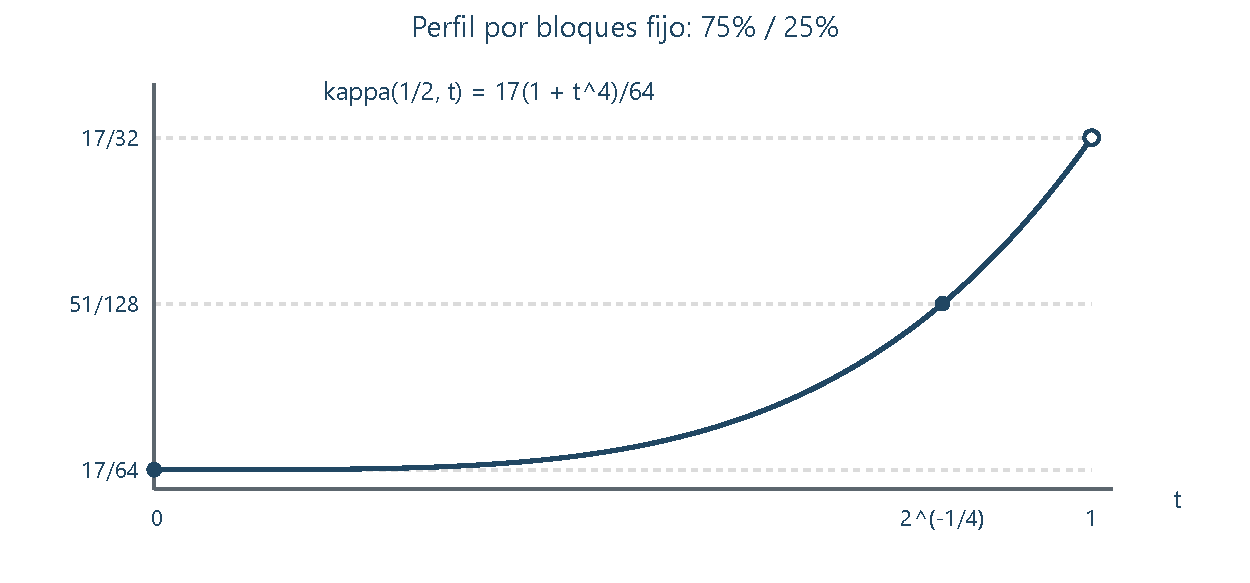
\includegraphics[width=0.94\linewidth]{figures/profile_es.pdf}
\caption{Coeficiente principal de intercalados para un perfil por bloques fijo. Se excluye el extremo t = 1; el teorema tiene un error aditivo y un umbral que depende de t.}
\end{figure}

\subsubsection{8.2. Cinco partes y triángulos arcoíris}\label{cinco-partes-y-triuxe1ngulos-arcouxedris}

Consideremos el grafo pentapartito completo \(K_{s,s,s,s,s}\), permitiendo precisamente los triángulos que encuentran tres clases distintas. Tiene \(5s\) vértices y \(10s^2\) aristas. Una descomposición en triángulos requiere \(3\mid10s^2\), de donde \(3\mid s\). Escribamos \(s=3m\).

\paragraph{8.2.1. Un testigo físico}\label{un-testigo-fuxedsico}

El apéndice B enumera treinta triángulos que descomponen \(K_{3,3,3,3,3}\). Sustituimos cada vértice de este grafo base por una copia de un grupo abeliano finito A de orden m. Sobre cada triángulo base elegimos las ternas de elementos del grupo que satisfacen \(x+y+z=0\).

Para una arista entre dos vértices expandidos de la base, el par de la base pertenece a un único triángulo base. Sus dos coordenadas de grupo determinan entonces la tercera de manera única. Por ello cada arista queda cubierta una vez, y los triángulos elevados dan una descomposición del grafo pentapartito con clases de tamaño \(3m\). Tomar \(A=\mathbb Z/m\mathbb Z\) proporciona todos los m positivos. Esto establece H2 mediante un testigo físico, sin recurrir a un criterio abstracto de divisibilidad.

\paragraph{8.2.2. Las hipótesis restantes y la conclusión}\label{las-hipuxf3tesis-restantes-y-la-conclusiuxf3n}

Por la completitud entre las partes, cada arista tiene exactamente \(3s\) vecinos comunes en las otras tres clases. El peso uniforme \(\mu(Q)=1/(3s)\) tiene sumas de aristas iguales a uno. Con orden del grafo ambiente \(5s\), H1 se cumple para \(C=5/3\): su cota difusa superior es \(1/(3s)\) y la inferior es menor.

Para cada tercera etiqueta compatible, un par tiene s vecinos comunes. El apéndice A da \((s-1)^2\) bisagras de orden seis. Por tanto, H3 y H4 se cumplen con \(\alpha=1/100\) y \(h=6\), pues para \(s\geq2\),
\[(s-1)^2\geq\frac{s^2}{4}=\frac1{100}(5s)^2.                        \tag{8.30}\]

\Needspace{7\baselineskip}\textbf{Corolario 8.5.} Fijemos \(\eta>0\) y un entero \(q\geq0\). Para todo entero m suficientemente grande, pongamos \(s=3m\). Para toda familia de a lo sumo \(s^q\) funciones de prueba con signo sobre los triángulos arcoíris de \(K_{s,s,s,s,s}\), cada una acotada en valor absoluto por uno, existe una descomposición arcoíris \(\mathcal D\) tal que
\[\left|\sum_{Q\in\mathcal D}w_j(Q)
-\frac1{3s}\sum_{Q\in\mathcal T}w_j(Q)\right|\leq\eta s^2          \tag{8.31}\]

para todo j, y
\[\left|P(\mathcal D)-\frac{|\mathcal P(\mathcal T)|}{(3s)^4}\right|
\leq\eta s^2.                                                       \tag{8.32}\]

\emph{Demostración.} La semilla uniforme verifica H1, la descomposición obtenida al expandir la base verifica H2, y el tamaño de las partes y el Apéndice A verifican H3 y H4. Aplicamos el Teorema T+ con precisión \(\eta/25\). El orden del grafo es \(5s\), por lo que el error se convierte en \(\eta s^2\). Cada Pasch contiene cuatro triángulos de peso \(1/(3s)\), lo que da (8.32).

La construcción base ya demuestra existencia en estos órdenes. La conclusión añadida es el control simultáneo de las estadísticas prescritas y del conteo de Pasch. Esta aplicación no requiere una expresión cerrada para \(|\mathcal P(\mathcal T)|\).

\subsection{9. Prueba formal y freeze auditado}\label{prueba-formal-y-freeze-auditado}

La prueba de T corresponde a \texttt{Typed\allowbreak{}Triangle.\allowbreak{}Vortex.\allowbreak{}main\_\allowbreak{}theorem\_\allowbreak{}T}, en \texttt{Main\allowbreak{}Paper\allowbreak{}III.\allowbreak{}lean}; el resultado conjunto corresponde a \texttt{Typed\allowbreak{}Triangle.\allowbreak{}Vortex.\allowbreak{}main\_\allowbreak{}theorem\_\allowbreak{}T\_\allowbreak{}with\_\allowbreak{}triangle\_\allowbreak{}monitors\_\allowbreak{}and\_\allowbreak{}pasch}, en \texttt{Main\allowbreak{}Paper\allowbreak{}IIIPasch.\allowbreak{}lean}. Los teoremas generales utilizan estas pruebas formales completas. Las secciones 3--6 y el apéndice D explican sus condiciones intermedias y su ensamblaje; no reproducen cada lema de construcción local como una prueba independiente en prosa.

El Teorema 8.4 dispone del resultado ensamblado \texttt{Typed\allowbreak{}Triangle.\allowbreak{}Applications.\allowbreak{}Latin.\allowbreak{}Two\allowbreak{}Scale.\allowbreak{}latin\_\allowbreak{}two\_\allowbreak{}scale\_\allowbreak{}with\_\allowbreak{}blocks}, en \texttt{Applications\allowbreak{}Two\allowbreak{}Scale\allowbreak{}Final.\allowbreak{}lean}. Construye los signos finos, demuestra la concentración simultánea, verifica la semilla y redondea ambos perfiles. Su corolario para la diferencia de conteos es \texttt{intercalate\_\allowbreak{}gap\_\allowbreak{}of\_\allowbreak{}targets}. La prueba utiliza la cota (8.24); la identidad finita exacta (8.23) se demuestra arriba y no se presenta como una identidad Lean ensamblada por separado.

El suplemento de fuentes tiene 1.141 módulos del proyecto y seis auditorías satisfactorias de axiomas de los resultados finales, que usan solo \texttt{propext}, \texttt{Classical.\allowbreak{}choice} y \texttt{Quot.\allowbreak{}sound}. El suplemento de formalización registra el SHA-256 del archivo, el manifiesto de fuentes, la reutilización validada de objetos y la recompilación de quince archivos en los que solo se actualizaron comentarios. El código matemático Lean y H1--H4 no cambiaron. Los resultados finales para perfiles y cuadrados latinos de una escala son \texttt{latin\_\allowbreak{}square\_\allowbreak{}with\_\allowbreak{}profile\_\allowbreak{}statistics}, \texttt{uniform\_\allowbreak{}with\_\allowbreak{}intercalates} y \texttt{signed\_\allowbreak{}profile\_\allowbreak{}with\_\allowbreak{}intercalates}, en el espacio de nombres \texttt{Typed\allowbreak{}Triangle.\allowbreak{}Applications.\allowbreak{}Latin}. El resultado pentapartito es \texttt{Typed\allowbreak{}Triangle.\allowbreak{}Applications.\allowbreak{}Five\allowbreak{}Partite.\allowbreak{}main\_\allowbreak{}theorem}. El suplemento de formalización enumera sus objetivos separados de compilación y sus consultas de auditoría.

\subsection{Agradecimientos}\label{agradecimientos}

El autor agradece profundamente a su esposa María Paz y a sus hijos Lucas, Juan Cristóbal, Francisca, Raimundo y Benjamín su amor, paciencia y apoyo.

\subsection{Uso de inteligencia artificial y herramientas computacionales}\label{uso-de-inteligencia-artificial-y-herramientas-computacionales}

Se utilizaron Claude, de Anthropic, y ChatGPT/Codex, de OpenAI, para explorar y revisar argumentos y preparar el manuscrito. Aristotle, de Harmonic, contribuyó a explorar enfoques, buscar contraejemplos, desarrollar demostraciones y formalizarlas y revisarlas en Lean. Su participación no se limitó a traducir pruebas terminadas.

Certo {[}16{]} y Jacobian {[}17{]} se utilizaron para explorar casos finitos, comprobar identidades y evaluar construcciones candidatas. Estos cálculos orientaron el desarrollo de los argumentos; las comprobaciones finitas no se trataron como pruebas de enunciados universales.

El autor es responsable de los argumentos, las citas, el código y la presentación. Ningún sistema de inteligencia artificial figura como autor.

\subsection{Apéndice A. Una bisagra física de seis vértices}\label{apuxe9ndice-a.-una-bisagra-fuxedsica-de-seis-vuxe9rtices}

El grafo subyacente es el octaedro \(K_{2,2,2}\) con partes \(\{u,x\}\), \(\{v,y\}\) y \(\{a,b\}\), retirando las dos caras raíz. Es la bisagra de 2-esfera de {[}14, Definición 14.3{]}, y pertenece a la construcción de intercambios octaédricos de {[}15, Sección 5.1{]}. Aquí damos su realización etiquetada y su conteo. Sean \(\{u,v,a\}\) y \(\{u,v,b\}\) triángulos arcoíris con \(a\ne b\). Elijamos x en la clase de u, con \(x\ne u\), e y en la clase de v, con \(y\ne v\). Definamos
\[J=\{uy,xv,xy,xa,xb,ya,yb\}.                                       \tag{A.1}\]

Los seis vértices son distintos. Las etiquetas de a y b pueden coincidir; ambas difieren de las etiquetas de u y v. Las aristas de J evitan los dos triángulos raíz. Sus dos descomposiciones son
\[\begin{aligned}
J\cup W_a&=E(\{u,y,a\})\,\dot\cup\,
 E(\{x,v,a\})\,\dot\cup\,E(\{x,y,b\}),\\
J\cup W_b&=E(\{u,y,b\})\,\dot\cup\,
 E(\{x,v,b\})\,\dot\cup\,E(\{x,y,a\}).
\end{aligned}                                                       \tag{A.2}\]

\begin{figure}[H]
\centering
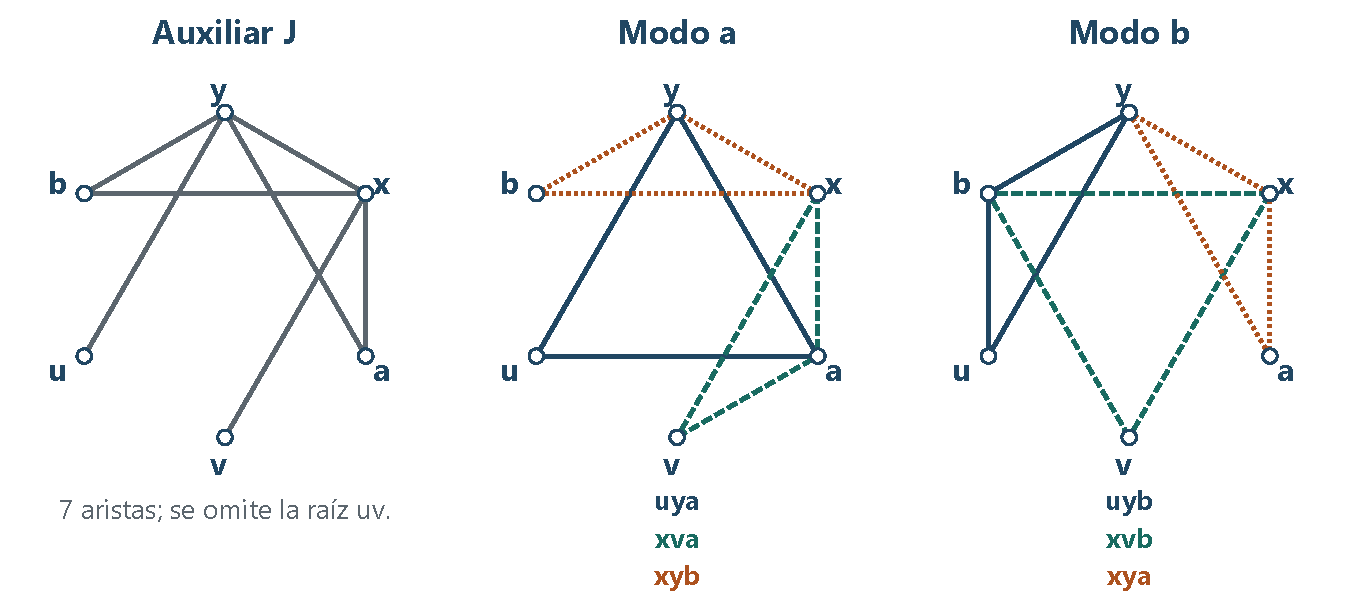
\includegraphics[width=0.98\linewidth]{figures/hinge_es.pdf}
\caption{Bisagra de seis vértices del apéndice A. El panel izquierdo muestra el grafo auxiliar J de siete aristas. Cada uno de los otros paneles divide J junto con una cuña en tres triángulos arcoíris, distinguidos por color y tipo de línea. Los cruces no son vértices. Este ejemplo corresponde a las aplicaciones multipartitas completas; H4 admite otras bisagras.}
\label{fig:hinge}
\end{figure}

Todos los triángulos mostrados son arcoíris. Expandir sus tres aristas verifica (A.2) y que esos conjuntos de aristas son disjuntos dos a dos. Cada uno de los seis vértices es incidente con J, por lo que el orden de la bisagra es seis.

Si cada clase tiene tamaño m, hay \((m-1)^2\) elecciones. Dan conjuntos de aristas distintos: recuperamos y como el único vecino de u en J, y x como el único vecino de v en J. Este es un conteo de bisagras físicas, sin dividir por una multiplicidad de etiquetado.

\subsection{Apéndice B. La base pentapartita de treinta bloques}\label{apuxe9ndice-b.-la-base-pentapartita-de-treinta-bloques}

Escribimos \(i_a\) para el vértice a de la clase i, donde \(i\in\{0,1,2,3,4\}\) y \(a\in\{0,1,2\}\). Las treinta ternas siguientes son el testigo base utilizado en la sección 8.2. Cada terna visita tres clases distintas. Cada par entre clases aparece exactamente una vez; la verificación finita también está registrada en el código fuente.

{\begin{longtable}[]{@{}lll@{}}
\toprule\noalign{}
\endhead
\bottomrule\noalign{}
\endlastfoot
\(\{0_0,1_0,4_0\}\) & \(\{0_1,2_1,4_2\}\) & \(\{1_0,3_0,4_1\}\) \\
\(\{0_0,1_1,3_2\}\) & \(\{0_1,3_1,4_0\}\) & \(\{1_1,2_1,4_0\}\) \\
\(\{0_0,1_2,2_1\}\) & \(\{0_2,1_0,3_1\}\) & \(\{1_1,2_2,3_0\}\) \\
\(\{0_0,2_0,4_1\}\) & \(\{0_2,1_1,2_0\}\) & \(\{1_1,3_1,4_2\}\) \\
\(\{0_0,2_2,3_1\}\) & \(\{0_2,1_2,4_2\}\) & \(\{1_2,2_0,3_1\}\) \\
\(\{0_0,3_0,4_2\}\) & \(\{0_2,2_1,3_0\}\) & \(\{1_2,2_2,4_1\}\) \\
\(\{0_1,1_0,2_2\}\) & \(\{0_2,2_2,4_0\}\) & \(\{1_2,3_2,4_0\}\) \\
\(\{0_1,1_1,4_1\}\) & \(\{0_2,3_2,4_1\}\) & \(\{2_0,3_0,4_0\}\) \\
\(\{0_1,1_2,3_0\}\) & \(\{1_0,2_0,4_2\}\) & \(\{2_1,3_1,4_1\}\) \\
\(\{0_1,2_0,3_2\}\) & \(\{1_0,2_1,3_2\}\) & \(\{2_2,3_2,4_2\}\) \\
\end{longtable}
}

Hay \(\binom52\cdot3^2=90\) aristas entre clases y treinta ternas, cada una con tres aristas. Comprobar la aparición de cada par verifica, por tanto, una descomposición exacta, no solo el número total correcto de bloques.

\Needspace{16\baselineskip}\subsection{Apéndice C. Identificación de la altura de la torre}\label{apuxe9ndice-c.-identificaciuxf3n-de-la-altura-de-la-torre}

La altura H de (7.6) se especifica mediante la siguiente composición de funciones sobre los naturales. Sus definiciones exactas se incluyen en la instantánea fija de fuentes y se identifican en la nota de formalización. Para evaluar la cota hacen falta esas definiciones; la composición mostrada no sustituye su desarrollo.
\[\begin{aligned}
h_*&=2h-3,\\
M&=\operatorname{triangleThresholdInputMajorant}(K,h,q),\\
A&=\operatorname{thresholdAgendaMajorant}(M),\\
R&=\operatorname{thresholdLayerScale}(A,h_*),\\
T&=\operatorname{thresholdTerminalScale}(R),\\
U&=\operatorname{thresholdReserveScale}(T,h_*),\\
H(K,h,q)&=\operatorname{triangleThresholdFinalMajorant}(U,h_*).
\end{aligned}                                                       \tag{C.1}\]

\subsection{Apéndice D. Estimaciones de preparación y cierre}\label{apuxe9ndice-d.-estimaciones-de-preparaciuxf3n-y-cierre}

Las constantes de este apéndice son locales a cada construcción. En particular, las cotas llamadas K y D no tienen por qué coincidir con la normalización K de (7.4) ni con las cotas de otra subsección. Conservamos la notación de cada estimación.

\subsubsection{D.1. Preparación y certificados}\label{d.1.-preparaciuxf3n-y-certificados}

Un núcleo preparado tiene cuatro propiedades después de cualquier eliminación de a lo sumo una fracción fija de sus vértices: disponibilidad de vecinos comunes y de bisagras, una cota inferior para el orden y persistencia del retículo entero físico. Son propiedades simultáneas de un mismo núcleo; no se vuelve a elegir el núcleo para cada demanda.

La persistencia se obtiene mediante el siguiente descenso finito. Supongamos que los cocientes físicos locales de una cadena de eliminaciones tienen rango a lo sumo d, torsión de orden a lo sumo T y aplicaciones de transición sobreyectivas. Leemos estas sobreyecciones del grafo menor al mayor, es decir, en sentido contrario al orden de eliminación. En esta dirección, a lo sumo d pasos disminuyen el rango. En un intervalo de rango constante, cada aplicación no inyectiva reduce el orden de la torsión por un factor de al menos dos. Por tanto, el número de pasos no inyectivos es a lo sumo
\[L=d+(d+1)\lfloor\log_2T\rfloor. \tag{D.1}\]

Fijemos un presupuesto b tal que todos los conjuntos de tamaño a lo sumo (L+1)b queden en el intervalo admisible. Si cada conjunto A de tamaño a lo sumo Lb admitiera otra eliminación de a lo sumo b vértices que causara falta de inyectividad, podríamos elegir esas eliminaciones sucesivamente desde el conjunto vacío. Tras j pasos, la unión tiene tamaño a lo sumo jb. Obtendríamos L+1 pasos no inyectivos, una contradicción. Existe entonces un A que sirve para todas las eliminaciones posteriores de a lo sumo b vértices. La restricción coloca cada demanda superviviente en el nuevo grupo local; la inyectividad conserva su pertenencia al retículo. Los lemas locales sobre cocientes y restricción forman parte de la construcción formal.

Detallamos el argumento de cocientes. Para un grafo J, sea \(M_J\) su grupo local de demandas enteras de aristas: las demandas se anulan fuera de J y, en cada vértice, la demanda incidente es una combinación entera de los vectores incidentes de triángulos permitidos. Sea \(\Lambda_J\) su retículo de triángulos. Cada vector de incidencia de un triángulo satisface estas condiciones locales, por lo que \(\Lambda_J\subseteq M_J\). Para grafos anidados \(J'\subseteq J\) con las mismas etiquetas, extender por cero los coeficientes de triángulos da inclusiones de ambos grupos. Por tanto, la inclusión induce \(M_{J'}/\Lambda_{J'}\longrightarrow M_J/\Lambda_J\). Su núcleo consta exactamente de las clases de demandas \(x\in M_{J'}\cap\Lambda_J\). Es inyectiva si y solo si \(M_{J'}\cap\Lambda_J=\Lambda_{J'}\): una demanda del retículo anterior que sigue siendo local en el grafo menor tiene un certificado allí.

La condición local debe comprobarse antes de utilizar esta igualdad. En la construcción la proporciona el resultado de ventanas locales bajo eliminaciones pequeñas, utilizado en \texttt{physical\_\allowbreak{}vertex\_\allowbreak{}first\_\allowbreak{}entry\_\allowbreak{}lattice} de \texttt{Vertex\allowbreak{}First\allowbreak{}Entry.\allowbreak{}lean}. El descenso finito da inyectividad uniformemente para toda eliminación posterior dentro del presupuesto. Estos dos hechos cumplen funciones distintas: el resultado de ventanas locales coloca la demanda superviviente en el grupo del dominio, y la inyectividad hace que su clase sea cero allí. El resultado geométrico de ventanas locales sigue siendo un lema de construcción del suplemento formal; la inyectividad por sí sola no lo sustituiría.

Por último, pasamos de eliminar las aristas incidentes con ciertos vértices al grafo inducido real. Extendemos por cero una demanda sobre los vértices supervivientes a todas las demás aristas. Extendemos del mismo modo un certificado de triángulos; su ecuación de incidencia se conserva porque cada triángulo solo utiliza vértices supervivientes. Si la demanda se anula además en otro conjunto que se elimina, también lo hace su extensión por cero. Aplicamos la persistencia en el conjunto ambiente de vértices y restringimos el certificado obtenido a los vértices restantes. Todos sus triángulos ya evitan los conjuntos eliminados, por lo que la restricción conserva cada ecuación de arista superviviente. Restringir la extensión por cero original devuelve la demanda original. Esto demuestra el transporte utilizado en \texttt{induced\_\allowbreak{}lattice\_\allowbreak{}persistence} de \texttt{Prepared\allowbreak{}Core\allowbreak{}Construction.\allowbreak{}lean}.

Un certificado acotado para una demanda que evita un conjunto prohibido se construye en el grafo superviviente y se extiende por cero. Se conservan su ecuación de incidencia y su norma. Para demandas simultáneas, sea K una cota de la norma de cada certificado y J su número; el tamaño prohibido admisible será al menos la mitad del presupuesto de preparación. Elegimos un entero q que cumpla
\[q\geq1,\qquad 6KJ\leq q\beta n. \tag{D.2}\]

Aquí \(\beta>0\) es la fracción permitida de borrado de vértices. El uso cuenta los certificados anteriores que contienen a v fuera de sus fronteras de demanda, una vez por certificado; no suma las multiplicidades de los coeficientes. Antes de cada elección se prohíben los vértices con uso al menos q, salvo los de la frontera actual. Un certificado de norma a lo sumo K encuentra como máximo 3K vértices, de modo que el uso total es a lo sumo 3KJ. La condición (D.2) deja prohibida a lo sumo la mitad del presupuesto de preparación. Existe el certificado siguiente, y cada uso auxiliar permanece a lo sumo en q. Si \(F_v\) cuenta las fronteras que contienen a v, sumar los certificados da
\[\|c\|_1\leq KJ,\qquad \operatorname{load}_v(c)\leq K(F_v+q). \tag{D.3}\]

Para obtener la cota numérica, usamos la elección \(q=\max\{1,\lceil6KJ/(\beta n)\rceil\}\) de la construcción de certificados, con \(\beta>0\) y \(n>0\). Esta satisface \(q\leq6KJ/(\beta n)+1\). Este parámetro local de carga es distinto del exponente q de T+. La frontera de una demanda es el conjunto de extremos de sus aristas no nulas. Las demandas encaminadas satisfacen la siguiente estimación de frontera, con \(\delta>0\) y \(D\geq0\). Sustituimos la cota de q en (D.3), usamos la cota de J y acotamos el techo restante por su argumento más uno. Los dos errores de redondeo dan el término aditivo de la última línea:
\[\begin{aligned}J&\leq2e,\quad e=\|x\|_1,\\ F_v&\leq(4D+3)d_{|x|}(v)+\left\lceil\frac{32De}{\delta n}\right\rceil+2D,\\ \operatorname{load}_v(c)&\leq K\left((4D+3)d_{|x|}(v)+\left(\frac{32D}{\delta}+\frac{12K}{\beta}\right)\frac e n+2D+2\right).\end{aligned}\tag{D.4}\]

\subsubsection{D.2. La semilla exacta corresponde al hijo real}\label{d.2.-la-semilla-exacta-corresponde-al-hijo-real}

Sea J el hijo efectivo después de los pagos y del recorte de la referencia, de orden \(n>0\). Supongamos \(\mathbf1_{E(J)}\in\Lambda_J\) y que \(\mu_0\) se anula fuera de sus triángulos permitidos. Tomemos \(C\geq1\), \(\varepsilon\geq0\) y una inversa suave de constante de norma K sobre la imagen real de \(A_J\). Las hipótesis restantes son \(1/(2Cn)\leq\mu_0(Q)\leq2C/n\) para Q permitido, \(\|r\|_\infty\leq\varepsilon\) para \(r=\mathbf1_{E(J)}-A_J\mu_0\), y \(K\varepsilon\leq1/(4C)\). La fisicalidad y el soporte sitúan r en la imagen real. La inversa proporciona entonces una corrección \(\xi\) con soporte permitido tal que
\[\begin{gathered}A_J\xi=r,\qquad |\xi(Q)|\leq\frac{K\varepsilon}{n},\\
A_J(\mu_0+\xi)=\mathbf1_{E(J)},\qquad \frac1{4Cn}\leq\mu_0(Q)+\xi(Q)\leq\frac{4C}{n}.\end{gathered}\tag{D.5}\]

La exactitud resulta de sumar las ecuaciones por arista. La cota inferior se obtiene restando el margen de corrección; para la superior se usa que C es al menos uno. La construcción proporciona el inverso y la semilla preliminar en este J. Un inverso del grafo original no demostraría esta afirmación.

\subsubsection{D.3. Una reserva elegida antes del residuo}\label{d.3.-una-reserva-elegida-antes-del-residuo}

Supongamos que la ventana terminal tiene a lo sumo u vértices. Enumeremos los residuos admisibles: conjuntos de aristas físicos soportados en esa ventana. Aquí disponibilidad robusta significa que cada residuo no vacío de este tipo tiene un absorbedor de a lo sumo s aristas que evita cualquier conjunto de aristas prohibidas dentro de un presupuesto fijo de grado máximo. La prueba de T usa el teorema de reserva uniforme \texttt{uniform\_\allowbreak{}terminal\_\allowbreak{}absorber\_\allowbreak{}avoiding\_\allowbreak{}outer\_\allowbreak{}core}; su versión con orden explícito se utiliza solo en la Sección 7. Coloquemos los absorbedores sucesivamente, prohibiendo el grafo protegido, todas las aristas de la ventana terminal y los absorbedores anteriores.
\[\#\{M\}\leq2^{u^2},\qquad |R|\leq s2^{u^2}. \tag{D.6}\]

El grado máximo prohibido queda acotado por el grado protegido más u y el tamaño indicado de la reserva. El umbral de orden hace que esta cantidad respete el presupuesto de suministro robusto. Los absorbedores tienen aristas disjuntas y evitan las aristas de la ventana terminal. Sus modos inactivos, que descomponen cada absorbedor sin añadir un residuo, descomponen conjuntamente R. Para un residuo posterior M, activamos su absorbedor y conservamos los demás en su modo inactivo. Así descomponemos la unión de R y M. La elección de R precedió a M.

\subsubsection{D.4. El coste de los Pasch que combinan etapas}\label{d.4.-el-coste-de-los-pasch-que-combinan-etapas}

Partimos de la familia disponible anterior, cuyo cogrado de pares es a lo sumo L. La nueva reserva de triángulos añade como máximo 1; el universo de retiros, 63; y los modos del banco, 2. Estas tres adiciones dan L+66. Añadir el nuevo empaquetamiento aporta a lo sumo uno más, lo que da L+67. Los pagos retirados y activados ya pertenecen a estas uniones. Los conteos de Pasch no tienen por qué sumarse entre las familias que las forman. La familia inicial de las etapas interiores es la salida de la capa exterior, que aplica esta estimación con una familia previa vacía: la reserva de triángulos, el universo de retiros, los modos del banco y el empaquetamiento dan \(1+63+2+1=67\). Esta es la cota que se pasa a \texttt{Tracking\allowbreak{}State.\allowbreak{}initial} desde \texttt{Pasch\allowbreak{}Concrete\allowbreak{}Outer\allowbreak{}Layer.\allowbreak{}lean} en \(j=0\); cada capa interior posterior añade a lo sumo 67, lo que da \(L\leq67+67j\).

Las estimaciones locales de inserción cargan cada Pasch nuevo a un triángulo modificado y acotan las tres elecciones restantes mediante un factor cúbico de cogrado de pares. Para cada unión ambiente sucesiva dan un coeficiente geométrico fijo multiplicado por \(nm_j(L+\ell)^3\), donde n es el orden original, \(m_j\) el orden actual y \(\ell\leq184\) un desplazamiento local. Sumemos esos coeficientes y llamemos G al resultado. Como \(L\leq67+67j\), (D.8) acota el cubo por \(318^3(j+1)^3\). La fuente define \(D=(|G|+1)318^3\), lo que da la cota de capa siguiente. Las estimaciones geométricas de inserción son los lemas formales locales ensamblados en \texttt{Pasch\allowbreak{}Concrete\allowbreak{}Inner\allowbreak{}Adaptive\allowbreak{}Layers.\allowbreak{}lean}; este argumento explica cómo sus cotas producen la recurrencia global.

El hijo siguiente contrae el orden al menos por un factor dieciséis. Definamos su margen restante mediante
\[\begin{gathered}16m_{j+1}\leq m_j,\qquad \Delta P_j\leq Dn(j+1)^3m_j,\\ \Phi_j=2Dn8^jm_j,\qquad (j+1)^3\leq8^j,\\ Dn(j+1)^3m_j+\Phi_{j+1}\leq Dn8^jm_j+16Dn8^jm_{j+1}\leq\Phi_j.\end{gathered}\tag{D.7}\]

La cota cúbica empieza con igualdad en j = 0. El paso inductivo se deduce de \((j+2)/(j+1)\leq2\). Además, al sustituir la definición de \(\Phi_{j+1}\) aparece el factor 16 de la última línea de (D.7); la contracción acota entonces ese término por \(Dn8^jm_j\). La desigualdad demuestra por inducción que el conteo actual de Pasch más el presupuesto restante nunca supera su presupuesto inicial. La constante D se fija antes del grafo. Su definición formal acota los incrementos de reserva, extracción, banco, empaquetamiento y cobertura en uniones ambientales consecutivas. El factor 318 procede de la cota de cogrado 67+67j y de un desplazamiento local máximo de 184:
\[L+184\leq251+67j\leq318(j+1).\tag{D.8}\]

Los desplazamientos numéricos de esta estimación proceden de cotas sobre uniones de familias disponibles de triángulos. Para cualquier par de vértices, el número de triángulos de una unión que contienen ese par es a lo sumo la suma de los números correspondientes en sus componentes; las coincidencias solo pueden reducirlo. Esto explica la suma de presupuestos de cogrado. En \texttt{Pasch\allowbreak{}Dense\allowbreak{}Weighted\allowbreak{}Withdrawal.\allowbreak{}lean}, el universo de extracción tiene cota 63, obtenida como 2+61. En \texttt{Pasch\allowbreak{}Concrete\allowbreak{}Structured\allowbreak{}Layer.\allowbreak{}lean} se combina con un empaquetamiento de cota 1. El banco aporta la cota adicional 2 indicada arriba. La prueba en \texttt{Pasch\allowbreak{}Concrete\allowbreak{}Inner\allowbreak{}Adaptive\allowbreak{}Layers.\allowbreak{}lean} acota sus desplazamientos intermedios por 184 y aplica después la estimación afín de cogrado. Sustituir la cota anterior 67+67j da (D.8). El valor 318 es un mayorante uniforme conveniente, no una nueva hipótesis de densidad. Estas cotas locales de familias son datos de la construcción formal; (D.7) explica cómo intervienen en el error global.

Detenemos el seguimiento cuando el orden actual es a lo sumo la raíz cuarta entera de n.~La parte final de la descomposición exacta, incluida la reserva terminal, añade a lo sumo K más el cuadrado de ese orden triángulos. Si n supera los dos techos siguientes, el número añadido es a lo sumo \(2\tau n\).
\[n\geq\lceil K/\tau\rceil,\quad n\geq\lceil1/\tau^2\rceil,\qquad K+m_j^2\leq2\tau n.\tag{D.9}\]

El punto de parada da \(m_j^2\leq\sqrt n\). La primera condición de orden da \(K\leq\tau n\); la segunda da \(\sqrt n\leq\tau n\), pues \(\tau>0\). Al sumar ambas cotas se obtiene (D.9).

\Needspace{25\baselineskip}Fijemos dos vértices distintos a y b de un triángulo raíz Q. En un Pasch que contiene Q, cada uno de a y b pertenece a exactamente otro triángulo, que llamamos A y B. Son distintos: de lo contrario, ese triángulo compartiría la arista ab con Q. Dos triángulos cualesquiera de un Pasch se cortan en exactamente un vértice. No pueden ser disjuntos: agotarían los seis vértices y un tercer triángulo podría cortar a cada uno en a lo sumo un vértice, dejando lugar para solo dos de sus tres vértices. Por tanto, A y B se cortan en un vértice x exterior a Q. En el empaquetamiento ambiente, el par ax determina A de manera única y bx determina B de manera única, pues una arista aparece en a lo sumo un triángulo. Los tres triángulos Q, A y B determinan el cuarto: deben pertenecer a él precisamente los tres vértices que todavía tienen grado uno. Así, dos Pasch enraizados a los que se asigna el mismo x son iguales. Esto inyecta las configuraciones enraizadas en los vértices exteriores a Q, dando a lo sumo n−3 configuraciones y, por tanto, la cota n utilizada aquí. Al cargar cada Pasch nuevo a su primer triángulo añadido, la contribución terminal queda acotada por \(2\tau n^2\). Combinando el error inicial \(\sigma\), el crecimiento seguido \(\tau\) y el error terminal \(2\tau\), obtenemos
\[|P(\mathcal D)-P_\mu|\leq(\sigma+3\tau)n^2=\eta n^2,\qquad \sigma=\tau=\eta/4.\tag{D.10}\]


\clearpage
\subsection{Referencias}\label{referencias}

\begingroup\small\raggedright\setlength{\parskip}{3pt}

{[}1{]} J. P. Traverso Gianini, \emph{Triangle decompositions I: Formalizing the Nash--Williams theorem in Lean}. Preprint 1.0, 20 de octubre de 2026. \href{https://doi.org/10.5281/zenodo.23428173}{doi:10.5281/zenodo.23428173}.

{[}2{]} J. P. Traverso Gianini, \emph{Triangle decompositions II: Robust absorption for typed triangles}. Preprint 1.0, 20 de octubre de 2026. \href{https://doi.org/10.5281/zenodo.23502224}{doi:10.5281/zenodo.23502224}.

{[}3{]} P. Keevash, \emph{Coloured and directed designs}. arXiv:1807.05770, versión 2, 2020. \href{https://arxiv.org/abs/1807.05770v2}{arXiv}.

{[}4{]} S. Ehard, S. Glock y F. Joos, \emph{Pseudorandom hypergraph matchings}. Combinatorics, Probability and Computing \textbf{29} (2020), 868--885. \href{https://doi.org/10.1017/S0963548320000280}{doi:10.1017/S0963548320000280}.

{[}5{]} J. P. Traverso Gianini, \emph{Formalizing Delcourt--Postle's refined absorption in Lean}. Nota de investigación, preprint 1.0.1, 27 de octubre de 2026. \href{https://doi.org/10.5281/zenodo.23715622}{doi:10.5281/zenodo.23715622}.

{[}6{]} M. Delcourt y L. Postle, \emph{Refined Absorption: A New Proof of the Existence Conjecture}. arXiv:2402.17855v1, 2024. \href{https://arxiv.org/abs/2402.17855v1}{arXiv}.

{[}7{]} L. Postle, \emph{Refined Absorption: A New Proof of the Existence Conjecture and its Applications to Extremal and Probabilistic Design Theory}. arXiv:2510.19978v1, 2025. \href{https://arxiv.org/abs/2510.19978v1}{arXiv}.

{[}8{]} F. Garbe, R. Hancock, J. Hladký y M. Sharifzadeh, \emph{Limits of Latin Squares}. Discrete Analysis \textbf{2023:8}. \href{https://doi.org/10.19086/da.83253}{doi:10.19086/da.83253}.

{[}9{]} M. Kwan, A. Sah y M. Sawhney, \emph{Large deviations in random Latin squares}. Bulletin of the London Mathematical Society \textbf{54} (2022), 1420--1438. \href{https://doi.org/10.1112/blms.12638}{doi:10.1112/blms.12638}.

{[}10{]} M. Kwan, A. Sah, M. Sawhney y M. Simkin, \emph{Substructures in Latin squares}. arXiv:2202.05088v4, 2022. \href{https://arxiv.org/abs/2202.05088v4}{arXiv}.

{[}11{]} B. Barber, D. Kühn, A. Lo, D. Osthus y A. Taylor, \emph{Clique decompositions of multipartite graphs and completion of Latin squares}. Journal of Combinatorial Theory, Series A \textbf{151} (2017), 146--201. \href{https://doi.org/10.1016/j.jcta.2017.04.005}{doi:10.1016/j.jcta.2017.04.005}.

{[}12{]} R. Montgomery, \emph{Fractional clique decompositions of dense partite graphs}. Combinatorics, Probability and Computing \textbf{26} (2017), 911--943. \href{https://doi.org/10.1017/S0963548317000165}{doi:10.1017/S0963548317000165}.

{[}13{]} M. Kwan y B. Sudakov, \emph{Intercalates and Discrepancy in Random Latin Squares}. arXiv:1607.04981v2, 2017. \href{https://arxiv.org/abs/1607.04981v2}{arXiv}.

{[}14{]} M. Delcourt y L. Postle, \emph{A Proof of Nash-Williams' Conjecture}. arXiv:2606.11178v1, 2026. \href{https://arxiv.org/abs/2606.11178v1}{arXiv}.

{[}15{]} P. Keevash, \emph{The existence of designs II}. arXiv:1802.05900v1, 2018. \href{https://arxiv.org/abs/1802.05900v1}{arXiv}.

{[}16{]} J. P. Traverso Gianini, \emph{Certo}, repositorio de software. \url{https://github.com/jtraverso/certo-math}.

{[}17{]} \emph{Jacobian}, repositorio de software. \url{https://github.com/morluto/jacobian}.

\endgroup

\end{document}
